% Written 2026-11-03 for Smith PHY 317 (Classical Mechanics), class 23 (Taylor 7.5, 7.8, 7.10),
% for a room that is about half physics/astronomy double majors. Companion to the three-springs
% handout in the 210 repo (MathematicalPhysics/CoupledDEs/ThreeSpringsHandout): same macros.tex,
% same shape (a credit line, a rule, then the highlights, result first and the steps after).
% The figure ueff_contours.pdf is drawn by make_figure.py in this folder.
% Build: latexmk -pdf AstroLagrange.tex.  Student copy: \masterfalse after %% Document setup for Syllabus and HW

\textwidth=7in
\textheight=9.5in
\topmargin=-1in
\headheight=0in
\headsep=.5in
\hoffset  -.85in

\usepackage{amsmath} % for \text{}
\usepackage{amsfonts} % For \text{}
\usepackage{amssymb} % For \text{}
\usepackage{amsthm}
\usepackage{bigints}

%% Stolen from Nathan Baker
\newcommand{\erf}{{\mathrm{erf}}}
\newcommand{\erfc}{{\mathrm{erfc}}}
\newcommand{\erfi}{{\mathrm{erfi}}}
\newcommand{\argh}{{\mathrm{arg}}}
\newcommand{\atan}{{\mathrm{atan}}}
\newcommand{\acos}{{\mathrm{acos}}}
\newcommand{\asin}{{\mathrm{asin}}}
\newcommand{\mat}[1]{\,\underline{\underline{#1}}\,}
\newcommand{\abs}[1]{\left| #1 \right|}
\newcommand{\norm}[1]{\left\| #1 \right\|}
\newcommand{\order}[1]{{\mathcal{O}} \left( #1 \right)}
\newcommand{\op}[1]{{\mathcal{#1}}}
\newcommand{\myfile}[1]{\texttt{#1}}
\newcommand{\myvar}[1]{\textsf{#1}}
\newcommand{\mean}[1]{{\left\langle {#1} \right\rangle}}

% The master boolean -- set this to "masterfalse" or "mastertrue"
%\newif\ifmaster \masterfalse
\newif\ifmaster \mastertrue

\newcommand{\hidesolution}[1]{ \ifmaster { {#1} } \else { {Go to class.} } \fi }
\newcommand{\hideanswer}[1]{ \ifmaster { #1 } \else {} \fi }
\newcommand{\solution}[1]{ \begin{proof}[Solution] \hidesolution{#1} \end{proof} }
\newcommand{\answer}[1]{ \hideanswer{\begin{proof}[Answer] #1 \end{proof}} }

%% MGL
\newcommand{\CC}{\mathbb{C}}
\newcommand{\N}{\mathbb{N}}
\newcommand{\Ham}{\mathcal{H}}
%\newcommand{\vect}[1]{\,\vec{\mathbf{#1}}\,}
\newcommand{\vect}[1]{\,\mathbf{#1}\,}
\usepackage{tabularx}
\newcommand{\vtau}{\vect{\tau}}
\newcommand{\vomega}{\vect{\omega}}
\newcommand{\va}{\vect{a}}
\newcommand{\vb}{\vect{b}}
\newcommand{\vc}{\vect{c}}
\newcommand{\vd}{\vect{d}}
\newcommand{\ve}{\vect{e}}
\newcommand{\vf}{\vect{f}}
\newcommand{\vg}{\vect{g}}
\newcommand{\vh}{\vect{h}}
\newcommand{\vi}{\vect{i}}
\newcommand{\vj}{\vect{j}}
\newcommand{\vk}{\vect{k}}
\newcommand{\vl}{\vect{l}}
\newcommand{\vm}{\vect{m}}
\newcommand{\vn}{\vect{n}}
\newcommand{\vo}{\vect{o}}
\newcommand{\vp}{\vect{p}}
\newcommand{\vq}{\vect{q}}
\newcommand{\vr}{\vect{r}}
\newcommand{\vs}{\vect{s}}
\newcommand{\vt}{\vect{t}}
\newcommand{\vu}{\vect{u}}
\newcommand{\vv}{\vect{v}}
\newcommand{\vw}{\vect{w}}
\newcommand{\vx}{\vect{x}}
\newcommand{\vy}{\vect{y}}
\newcommand{\vz}{\vect{z}}

\newcommand{\vA}{\vect{A}}
\newcommand{\vB}{\vect{B}}
\newcommand{\vC}{\vect{C}}
\newcommand{\vD}{\vect{D}}
\newcommand{\vE}{\vect{E}}
\newcommand{\vF}{\vect{F}}
\newcommand{\vG}{\vect{G}}
\newcommand{\vH}{\vect{H}}
\newcommand{\vI}{\vect{I}}
\newcommand{\vJ}{\vect{J}}
\newcommand{\vK}{\vect{K}}
\newcommand{\vL}{\vect{L}}
\newcommand{\vM}{\vect{M}}
\newcommand{\vN}{\vect{N}}
\newcommand{\vO}{\vect{O}}
\newcommand{\vP}{\vect{P}}
\newcommand{\vQ}{\vect{Q}}
\newcommand{\vR}{\vect{R}}
\newcommand{\vS}{\vect{S}}
\newcommand{\vT}{\vect{T}}
\newcommand{\vU}{\vect{U}}
\newcommand{\vV}{\vect{V}}
\newcommand{\vW}{\vect{W}}
\newcommand{\vX}{\vect{X}}
\newcommand{\vY}{\vect{Y}}
\newcommand{\vZ}{\vect{Z}}
%\newcommand{\pd}[2]{\frac{\partial#1}{\partial#2}}
%\newcommand{\dd}[2]{\frac{d#1}{d#2}}
\newcommand{\dinline}[2]{d #1/d #2} % for derivatives
\newcommand{\pdinline}[2]{\partial#1/\partial#2}

\newcommand{\boldcent}[1] {\begin{center}\textbf{ #1 }\end{center}}
% ***********************************************************
% ******************* PHYSICS HEADER ************************
% ***********************************************************
% From http://www.dfcd.net/articles/latex/latex.html
% Version 2
%\documentclass[11pt]{article} 
\usepackage{amsmath} % AMS Math Package
\usepackage{amsthm} % Theorem Formatting
\usepackage{amssymb}	% Math symbols such as \mathbb
\usepackage{graphicx} % Allows for eps images
\usepackage{multicol} % Allows for multiple columns
%\usepackage[dvips,letterpaper,margin=0.75in,bottom=0.5in]{geometry}
% % Sets margins and page size
%\pagestyle{empty} % Removes page numbers
%\makeatletter % Need for anything that contains an @ command 
%\renewcommand{\maketitle} % Redefine maketitle to conserve space
%{ \begingroup \vskip 10pt \begin{center} \large {\bf \@title}
%	\vskip 10pt \large \@author \hskip 20pt \@date \end{center}
%  \vskip 10pt \endgroup \setcounter{footnote}{0} }
%\makeatother % End of region containing @ commands
\renewcommand{\labelenumi}{(\alph{enumi})} % Use letters for enumerate
% \DeclareMathOperator{\Sample}{Sample}
\let\vaccent=\v % rename builtin command \v{} to \vaccent{}
\renewcommand{\v}[1]{\ensuremath{\mathbf{#1}}} % for vectors
\newcommand{\gv}[1]{\ensuremath{\mbox{\boldmath$ #1 $}}} 
% for vectors of Greek letters
\newcommand{\uv}[1]{\ensuremath{\mathbf{\hat{#1}}}} % for unit vector
%\newcommand{\abs}[1]{\left| #1 \right|} % for absolute value
\newcommand{\avg}[1]{\left< #1 \right>} % for average
%\let\underdot=\d % rename builtin command \d{} to \underdot{}
%\renewcommand{\d}[2]{\frac{d #1}{d #2}} % for derivatives
\newcommand{\fd}[2]{\frac{d #1}{d #2}} % for derivatives
\newcommand{\dd}[2]{\frac{d^2 #1}{d #2^2}} % for double derivatives
\newcommand{\pd}[2]{\frac{\partial #1}{\partial #2}} 
% for partial derivatives
\newcommand{\pdd}[2]{\frac{\partial^2 #1}{\partial #2^2}} 
\newcommand{\pddx}[3]{\frac{\partial^2 #1}{\partial #2 \partial #3}} 
% for double partial derivatives
\newcommand{\pdc}[3]{\left( \frac{\partial #1}{\partial #2}
 \right)_{#3}} % for thermodynamic partial derivatives
\newcommand{\ket}[1]{\left| #1 \right>} % for Dirac bras
\newcommand{\bra}[1]{\left< #1 \right|} % for Dirac kets
\newcommand{\braket}[2]{\left< #1 \vphantom{#2} \right|
 \left. #2 \vphantom{#1} \right>} % for Dirac brackets
\newcommand{\matrixel}[3]{\left< #1 \vphantom{#2#3} \right|
 #2 \left| #3 \vphantom{#1#2} \right>} % for Dirac matrix elements
\newcommand{\grad}[1]{\gv{\nabla} #1} % for gradient
\let\divsymb=\div % rename builtin command \div to \divsymb
\renewcommand{\div}[1]{\gv{\nabla} \cdot #1} % for divergence
\newcommand{\tdiv}[1]{\text{div} #1} % for divergence
\newcommand{\curl}[1]{\gv{\nabla} \times #1} % for curl
\newcommand{\lap}[1]{\gv{\nabla}^{2} #1} % for gradient
\let\baraccent=\= % rename builtin command \= to \baraccent
\renewcommand{\=}[1]{\stackrel{#1}{=}} % for putting numbers above =
\newtheorem{prop}{Proposition}
\newtheorem{thm}{Theorem}[section]
\newtheorem{lem}[thm]{Lemma}
\theoremstyle{definition}
\newtheorem{dfn}{Definition}
\theoremstyle{remark}
\newtheorem*{rmk}{Remark}

% ***********************************************************
% ********************** END HEADER *************************
% ***********************************************************

%% Labelled matrices, Felder and Felder style (column labels above the
%% parentheses, row labels to the left). Built on plain TeX's \bordermatrix.
%%   \lmat{col1}{col2}{row1}{row2}{a}{b}{c}{d}   a 2x2 with labels
%%   \lmatt{c1}{c2}{c3}{r1}{r2}{r3}{a}{b}{c}{d}{e}{f}{g}{h}{i} is one argument
%%   too many for \newcommand, so for 3x3 and up write \bordermatrix directly:
%%   \bordermatrix{ & c1 & c2 & c3 \cr r1 & a & b & c \cr r2 & d & e & f \cr r3 & g & h & i }
\newcommand{\lmat}[8]{\bordermatrix{ & #1 & #2 \cr #3 & #5 & #6 \cr #4 & #7 & #8 }}
.
\documentclass[12pt]{article}
%% Document setup for Syllabus and HW

\textwidth=7in
\textheight=9.5in
\topmargin=-1in
\headheight=0in
\headsep=.5in
\hoffset  -.85in

\usepackage{amsmath} % for \text{}
\usepackage{amsfonts} % For \text{}
\usepackage{amssymb} % For \text{}
\usepackage{amsthm}
\usepackage{bigints}

%% Stolen from Nathan Baker
\newcommand{\erf}{{\mathrm{erf}}}
\newcommand{\erfc}{{\mathrm{erfc}}}
\newcommand{\erfi}{{\mathrm{erfi}}}
\newcommand{\argh}{{\mathrm{arg}}}
\newcommand{\atan}{{\mathrm{atan}}}
\newcommand{\acos}{{\mathrm{acos}}}
\newcommand{\asin}{{\mathrm{asin}}}
\newcommand{\mat}[1]{\,\underline{\underline{#1}}\,}
\newcommand{\abs}[1]{\left| #1 \right|}
\newcommand{\norm}[1]{\left\| #1 \right\|}
\newcommand{\order}[1]{{\mathcal{O}} \left( #1 \right)}
\newcommand{\op}[1]{{\mathcal{#1}}}
\newcommand{\myfile}[1]{\texttt{#1}}
\newcommand{\myvar}[1]{\textsf{#1}}
\newcommand{\mean}[1]{{\left\langle {#1} \right\rangle}}

% The master boolean -- set this to "masterfalse" or "mastertrue"
%\newif\ifmaster \masterfalse
\newif\ifmaster \mastertrue

\newcommand{\hidesolution}[1]{ \ifmaster { {#1} } \else { {Go to class.} } \fi }
\newcommand{\hideanswer}[1]{ \ifmaster { #1 } \else {} \fi }
\newcommand{\solution}[1]{ \begin{proof}[Solution] \hidesolution{#1} \end{proof} }
\newcommand{\answer}[1]{ \hideanswer{\begin{proof}[Answer] #1 \end{proof}} }

%% MGL
\newcommand{\CC}{\mathbb{C}}
\newcommand{\N}{\mathbb{N}}
\newcommand{\Ham}{\mathcal{H}}
%\newcommand{\vect}[1]{\,\vec{\mathbf{#1}}\,}
\newcommand{\vect}[1]{\,\mathbf{#1}\,}
\usepackage{tabularx}
\newcommand{\vtau}{\vect{\tau}}
\newcommand{\vomega}{\vect{\omega}}
\newcommand{\va}{\vect{a}}
\newcommand{\vb}{\vect{b}}
\newcommand{\vc}{\vect{c}}
\newcommand{\vd}{\vect{d}}
\newcommand{\ve}{\vect{e}}
\newcommand{\vf}{\vect{f}}
\newcommand{\vg}{\vect{g}}
\newcommand{\vh}{\vect{h}}
\newcommand{\vi}{\vect{i}}
\newcommand{\vj}{\vect{j}}
\newcommand{\vk}{\vect{k}}
\newcommand{\vl}{\vect{l}}
\newcommand{\vm}{\vect{m}}
\newcommand{\vn}{\vect{n}}
\newcommand{\vo}{\vect{o}}
\newcommand{\vp}{\vect{p}}
\newcommand{\vq}{\vect{q}}
\newcommand{\vr}{\vect{r}}
\newcommand{\vs}{\vect{s}}
\newcommand{\vt}{\vect{t}}
\newcommand{\vu}{\vect{u}}
\newcommand{\vv}{\vect{v}}
\newcommand{\vw}{\vect{w}}
\newcommand{\vx}{\vect{x}}
\newcommand{\vy}{\vect{y}}
\newcommand{\vz}{\vect{z}}

\newcommand{\vA}{\vect{A}}
\newcommand{\vB}{\vect{B}}
\newcommand{\vC}{\vect{C}}
\newcommand{\vD}{\vect{D}}
\newcommand{\vE}{\vect{E}}
\newcommand{\vF}{\vect{F}}
\newcommand{\vG}{\vect{G}}
\newcommand{\vH}{\vect{H}}
\newcommand{\vI}{\vect{I}}
\newcommand{\vJ}{\vect{J}}
\newcommand{\vK}{\vect{K}}
\newcommand{\vL}{\vect{L}}
\newcommand{\vM}{\vect{M}}
\newcommand{\vN}{\vect{N}}
\newcommand{\vO}{\vect{O}}
\newcommand{\vP}{\vect{P}}
\newcommand{\vQ}{\vect{Q}}
\newcommand{\vR}{\vect{R}}
\newcommand{\vS}{\vect{S}}
\newcommand{\vT}{\vect{T}}
\newcommand{\vU}{\vect{U}}
\newcommand{\vV}{\vect{V}}
\newcommand{\vW}{\vect{W}}
\newcommand{\vX}{\vect{X}}
\newcommand{\vY}{\vect{Y}}
\newcommand{\vZ}{\vect{Z}}
%\newcommand{\pd}[2]{\frac{\partial#1}{\partial#2}}
%\newcommand{\dd}[2]{\frac{d#1}{d#2}}
\newcommand{\dinline}[2]{d #1/d #2} % for derivatives
\newcommand{\pdinline}[2]{\partial#1/\partial#2}

\newcommand{\boldcent}[1] {\begin{center}\textbf{ #1 }\end{center}}
% ***********************************************************
% ******************* PHYSICS HEADER ************************
% ***********************************************************
% From http://www.dfcd.net/articles/latex/latex.html
% Version 2
%\documentclass[11pt]{article} 
\usepackage{amsmath} % AMS Math Package
\usepackage{amsthm} % Theorem Formatting
\usepackage{amssymb}	% Math symbols such as \mathbb
\usepackage{graphicx} % Allows for eps images
\usepackage{multicol} % Allows for multiple columns
%\usepackage[dvips,letterpaper,margin=0.75in,bottom=0.5in]{geometry}
% % Sets margins and page size
%\pagestyle{empty} % Removes page numbers
%\makeatletter % Need for anything that contains an @ command 
%\renewcommand{\maketitle} % Redefine maketitle to conserve space
%{ \begingroup \vskip 10pt \begin{center} \large {\bf \@title}
%	\vskip 10pt \large \@author \hskip 20pt \@date \end{center}
%  \vskip 10pt \endgroup \setcounter{footnote}{0} }
%\makeatother % End of region containing @ commands
\renewcommand{\labelenumi}{(\alph{enumi})} % Use letters for enumerate
% \DeclareMathOperator{\Sample}{Sample}
\let\vaccent=\v % rename builtin command \v{} to \vaccent{}
\renewcommand{\v}[1]{\ensuremath{\mathbf{#1}}} % for vectors
\newcommand{\gv}[1]{\ensuremath{\mbox{\boldmath$ #1 $}}} 
% for vectors of Greek letters
\newcommand{\uv}[1]{\ensuremath{\mathbf{\hat{#1}}}} % for unit vector
%\newcommand{\abs}[1]{\left| #1 \right|} % for absolute value
\newcommand{\avg}[1]{\left< #1 \right>} % for average
%\let\underdot=\d % rename builtin command \d{} to \underdot{}
%\renewcommand{\d}[2]{\frac{d #1}{d #2}} % for derivatives
\newcommand{\fd}[2]{\frac{d #1}{d #2}} % for derivatives
\newcommand{\dd}[2]{\frac{d^2 #1}{d #2^2}} % for double derivatives
\newcommand{\pd}[2]{\frac{\partial #1}{\partial #2}} 
% for partial derivatives
\newcommand{\pdd}[2]{\frac{\partial^2 #1}{\partial #2^2}} 
\newcommand{\pddx}[3]{\frac{\partial^2 #1}{\partial #2 \partial #3}} 
% for double partial derivatives
\newcommand{\pdc}[3]{\left( \frac{\partial #1}{\partial #2}
 \right)_{#3}} % for thermodynamic partial derivatives
\newcommand{\ket}[1]{\left| #1 \right>} % for Dirac bras
\newcommand{\bra}[1]{\left< #1 \right|} % for Dirac kets
\newcommand{\braket}[2]{\left< #1 \vphantom{#2} \right|
 \left. #2 \vphantom{#1} \right>} % for Dirac brackets
\newcommand{\matrixel}[3]{\left< #1 \vphantom{#2#3} \right|
 #2 \left| #3 \vphantom{#1#2} \right>} % for Dirac matrix elements
\newcommand{\grad}[1]{\gv{\nabla} #1} % for gradient
\let\divsymb=\div % rename builtin command \div to \divsymb
\renewcommand{\div}[1]{\gv{\nabla} \cdot #1} % for divergence
\newcommand{\tdiv}[1]{\text{div} #1} % for divergence
\newcommand{\curl}[1]{\gv{\nabla} \times #1} % for curl
\newcommand{\lap}[1]{\gv{\nabla}^{2} #1} % for gradient
\let\baraccent=\= % rename builtin command \= to \baraccent
\renewcommand{\=}[1]{\stackrel{#1}{=}} % for putting numbers above =
\newtheorem{prop}{Proposition}
\newtheorem{thm}{Theorem}[section]
\newtheorem{lem}[thm]{Lemma}
\theoremstyle{definition}
\newtheorem{dfn}{Definition}
\theoremstyle{remark}
\newtheorem*{rmk}{Remark}

% ***********************************************************
% ********************** END HEADER *************************
% ***********************************************************

%% Labelled matrices, Felder and Felder style (column labels above the
%% parentheses, row labels to the left). Built on plain TeX's \bordermatrix.
%%   \lmat{col1}{col2}{row1}{row2}{a}{b}{c}{d}   a 2x2 with labels
%%   \lmatt{c1}{c2}{c3}{r1}{r2}{r3}{a}{b}{c}{d}{e}{f}{g}{h}{i} is one argument
%%   too many for \newcommand, so for 3x3 and up write \bordermatrix directly:
%%   \bordermatrix{ & c1 & c2 & c3 \cr r1 & a & b & c \cr r2 & d & e & f \cr r3 & g & h & i }
\newcommand{\lmat}[8]{\bordermatrix{ & #1 & #2 \cr #3 & #5 & #6 \cr #4 & #7 & #8 }}


\usepackage[utf8]{inputenc}
\usepackage{tikz}
\usepackage{booktabs}
\usepackage[colorlinks=true, linkcolor=blue, citecolor=blue, urlcolor=blue]{hyperref}
\numberwithin{equation}{section}

\newcommand{\Om}{\Omega}
\newcommand{\Lag}{\mathcal{L}}
\newcommand{\Ueff}{U_{\rm eff}}
\newcommand{\vpec}{v_{\rm pec}}

\begin{document}
\title{Highlights from two astronomy problems for Lagrange's equations: \\
  the cosmological redshift and the Lagrange points}
\author{Michael G. Lerner}
\date{\today}

\maketitle

These notes use only what is in Taylor, \emph{Classical Mechanics}, Sections 7.1, 7.3, 7.5, 7.6 and 7.8:
Hamilton's principle, Lagrange's equations, constraints and degrees of freedom, a coordinate change that depends on time, ignorable coordinates, and
``no $t$ in $\Lag$ gives a conserved Hamiltonian.'' The cosmology half follows the standard
textbook route for a particle in an expanding universe (P.~J.~E. Peebles, \emph{The Large-Scale
Structure of the Universe}, Princeton, 1980, Chapter~II); the second half is the restricted
three-body problem as every celestial-mechanics book sets it up (e.g.\ Murray and Dermott,
\emph{Solar System Dynamics}, Cambridge, 1999, Chapter~3; the Lagrangian route is the one in
Goldstein, Poole and Safko, \emph{Classical Mechanics}, 3rd ed., Section~3.12). Both halves are Newtonian
throughout, and the places where general relativity would add something are flagged.

\setlength{\unitlength}{1in}

\noindent\begin{picture}(7,.1)
\put(0,0) {\line(1,0){7}}
\end{picture}

\section{The redshift: Noether in an expanding universe}
\label{sec:redshift}

\noindent\emph{This is the long version, result first. Section~\ref{sec:redshift-straight} does the
same problem straight through, in the order every Chapter~7 problem goes.}

\noindent\textbf{The setup.} Hubble's law says a galaxy at distance $r$ recedes from us at
$v = (\dot a/a)\, r$, where $a(t)$ is the \emph{scale factor}: every cosmological distance
grows as $r(t) = a(t)\, x$, with $x$ a label that does not change. Coordinates that expand
with the universe like this are called \emph{comoving coordinates}: a galaxy that just rides
the expansion (the ``Hubble flow'') sits at a fixed $x$ forever. Differentiating,
\begin{equation}
  \dot r = \dot a\, x + a\, \dot x ,
\end{equation}
the Hubble flow $\dot a\,x = (\dot a/a)\,r$ (using $x = r/a$; Hubble's law: the whole motion when $\dot x = 0$) plus the \emph{peculiar velocity} $\vpec \equiv a\dot x$, the motion relative
to the flow (a galaxy falling toward a cluster, say, or a photon crossing the universe).

\medskip

\noindent\textbf{The result, first.} For a particle moving freely through a homogeneous
expanding universe, in comoving coordinates,
\begin{equation}
  \label{eq:Lcosmo}
  \boxed{\;\Lag = \tfrac12\, m\, a(t)^2\, \dot x^2\;}
  \qquad\text{(up to a total time derivative, which changes nothing; see Step~3).}
\end{equation}
Two things follow immediately from Taylor's Sections~7.6 (ignorable coordinates) and 7.8 (the
Hamiltonian); both are cases of Noether's theorem, that each symmetry of $\Lag$ gives a
conserved quantity:
\begin{itemize}
\item $x$ does not appear in $\Lag$, so Lagrange's equation for $x$,
  $\frac{d}{dt}\,\partial\Lag/\partial\dot x = \partial\Lag/\partial x = 0$, reads
  $\frac{d}{dt}(m a^2\dot x) = 0$: the coordinate is ignorable and
  $p \equiv \partial\Lag/\partial\dot x = m a^2 \dot x$ is conserved. In terms of the peculiar
  velocity, $p = m a\,(a\dot x) = m\, a\, \vpec$ is constant, so
  \begin{equation}
    \label{eq:hubbledrag}
    \vpec \propto \frac{1}{a} .
  \end{equation}
  Random motions die away as the universe grows (``Hubble drag''): when the universe doubles in
  size, every freely coasting peculiar velocity halves.
\item $t$ \emph{does} appear in $\Lag$, through $a(t)$, so there is no conserved Hamiltonian
  and no conserved energy (for any particle with $\vpec \neq 0$; one riding the flow has
  $\Ham = 0$ throughout). The expanding universe does not have time-translation symmetry, and
  Noether's theorem has nothing to give.
\end{itemize}
The rest of this section is where \eqref{eq:Lcosmo} comes from, and then what it says about
light.

\medskip

\noindent\textbf{Step 1: Newton's law for the expansion.} Fill space with matter of uniform
density $\rho(t)$. Pick any point as the origin. A particle at $r$ feels only the gravity of
the sphere inside it (Newton's shell theorem: a uniform spherical shell pulls on a particle outside it as if all its
mass sat at its center, and exerts no net force on a particle inside it; that the outside cancels is the one place
Newtonian cosmology has to wave its hands, and general relativity makes the argument honest),
so Newton's second law for the particle, $m\ddot r = -G m M(<r)/r^2$, divided by $m$, gives
\begin{equation}
  \ddot r = -\frac{G M(<r)}{r^2} = -\frac{G}{r^2}\cdot\frac{4\pi}{3}\rho r^3
  = -\frac{4\pi G}{3}\,\rho\, r ,
  \qquad\text{i.e.}\qquad
  \Phi(r) = \frac{2\pi G}{3}\,\rho\, r^2 .
\end{equation}
Here $M(<r)$ is the mass inside radius $r$, and $\Phi$ is the gravitational potential energy per
unit mass, chosen so that $\ddot r = -d\Phi/dr$. A particle riding the Hubble flow has $r = a x$
with $x$ constant, so $\ddot r = \ddot a\, x$, and the force law above with $r = a x$ reads
$\ddot a\, x = -\frac{4\pi G}{3}\rho\,a x$; cancelling $x$,
\begin{equation}
  \label{eq:friedmann}
  \ddot a = -\frac{4\pi G}{3}\,\rho\, a .
\end{equation}
This is the Friedmann acceleration equation for a universe of pressureless matter. (General
relativity's version has extra terms for pressure and for the cosmological constant; with those
set to zero it is exactly this.)

\medskip

\noindent\textbf{Step 2: the Lagrangian in comoving coordinates.} Work in one dimension; three
is the same with vectors. A particle that is \emph{not} riding the flow has $r = a x$ with
$x(t)$ free. This is a time-dependent coordinate change, as in Section~7.5: $a(t)$ is a given
function of time that obeys \eqref{eq:friedmann}, not a coordinate, and $x$ is the only
generalized coordinate. Then
\begin{align}
  \Lag = \tfrac12 m\dot r^2 - m\Phi
  &= \tfrac12 m\,(\dot a x + a\dot x)^2 - \frac{2\pi G}{3}\, m \rho\, a^2 x^2 \nonumber\\
  &= \tfrac12 m a^2\dot x^2 \;+\; m a\dot a\, x\dot x \;+\; \tfrac12 m\dot a^2 x^2
     \;-\; \frac{2\pi G}{3}\, m\rho\, a^2 x^2 .
  \label{eq:Lexpanded}
\end{align}
The cross term is the one to tame. Since $\frac{d}{dt}\bigl(\tfrac12 m a\dot a\, x^2\bigr)
= \tfrac12 m(\dot a^2 + a\ddot a)\,x^2 + m a\dot a\, x\dot x$ (product rule, with
$\frac{d}{dt}(a\dot a) = \dot a^2 + a\ddot a$ and $\frac{d}{dt}x^2 = 2x\dot x$), solving for the cross term gives
\begin{equation}
  m a\dot a\, x\dot x = \frac{d}{dt}\Bigl(\tfrac12 m a\dot a\, x^2\Bigr)
  - \tfrac12 m\dot a^2 x^2 - \tfrac12 m a\ddot a\, x^2 .
\end{equation}
Put that into \eqref{eq:Lexpanded}:
\begin{equation}
  \Lag = \tfrac12 m a^2\dot x^2 + \frac{d}{dt}\Bigl(\tfrac12 m a\dot a\, x^2\Bigr)
  - \tfrac12 m\dot a^2 x^2 - \tfrac12 m a\ddot a\, x^2
  + \tfrac12 m\dot a^2 x^2 - \frac{2\pi G}{3}\, m\rho\, a^2 x^2 .
\end{equation}
The two $\tfrac12 m\dot a^2 x^2$ terms cancel, and by
\eqref{eq:friedmann}, $\ddot a = -\frac{4\pi G}{3}\rho\,a$, the $-\tfrac12 m a\ddot a\,x^2$ term is $-\tfrac12 m a\ddot a\,x^2 = +\frac{2\pi G}{3} m\rho a^2 x^2$, which
cancels the potential term exactly. What is left is
\begin{equation}
  \Lag = \tfrac12 m a^2\dot x^2 + \frac{dF}{dt}, \qquad F \equiv \tfrac12 m a\dot a\, x^2 .
\end{equation}

\medskip

\noindent\textbf{Step 3: a total derivative in $\Lag$ changes nothing.} The action is
$S = \int_{t_1}^{t_2}\Lag\,dt$, and $\int_{t_1}^{t_2} (dF/dt)\,dt = F(t_2) - F(t_1)$ is fixed
by the endpoints ($F = \tfrac12 m a\dot a\,x^2$ depends only on $x$ and $t$, and Hamilton's
principle, Section~7.1, varies paths with $x(t_1)$ and $x(t_2)$ held fixed): it is the same
number for every path between them, so it cannot change which
path makes $S$ stationary. (Check: put $\Lag = dF/dt = \partial_t F + \dot x\,\partial_x F$
into Lagrange's equation by itself: $\partial\Lag/\partial\dot x = \partial_x F$, so
$\frac{d}{dt}\,\partial\Lag/\partial\dot x = \partial_t\partial_x F + \dot x\,\partial_x^2 F$,
which is exactly $\partial\Lag/\partial x = \partial_x\partial_t F + \dot x\,\partial_x^2 F$ (mixed partial derivatives are equal), and the equation reads $0 = 0$.) So we may drop it, and
\eqref{eq:Lcosmo} is the Lagrangian. Had there been lumps in the universe, a galaxy cluster
say, \eqref{eq:Lcosmo} would pick up $-m\phi(x,t)$ with $\phi$ the \emph{peculiar} potential
of the lumps alone; that is Peebles's starting point for structure formation. The smooth background's potential
vanished here because the expansion already accounts for it: in Step~2 it cancelled against the
$a\ddot a$ term, through \eqref{eq:friedmann}.

\medskip

\noindent\textbf{The Hamiltonian, and what is not conserved.} With \eqref{eq:Lcosmo} (the total derivative dropped) and $p = m a^2\dot x$,
\begin{equation}
  \Ham = p\dot x - \Lag = m a^2\dot x^2 - \tfrac12 m a^2\dot x^2 = \tfrac12 m (a\dot x)^2 = \tfrac12 m\vpec^2 ,
\end{equation}
which is the kinetic energy in the peculiar velocity, and Taylor's general result
$d\Ham/dt = -\partial\Lag/\partial t$ (Section~7.8), with $\partial\Lag/\partial t = m a\dot a\,\dot x^2$
($\Lag$ depends on $t$ only through $a$), gives
\begin{equation}
  \frac{d\Ham}{dt} = -m a\dot a\,\dot x^2 = -2\,\frac{\dot a}{a}\,\Ham ,
  \qquad\text{so}\qquad \Ham \propto \frac{1}{a^2},
\end{equation}
consistent with \eqref{eq:hubbledrag}, since $\Ham = \tfrac12 m\vpec^2$ and $\vpec \propto 1/a$.
(The middle step is $m a\dot a\,\dot x^2 = (2\dot a/a)\cdot\tfrac12 m a^2\dot x^2$, and
$d\ln\Ham/dt = -2\,d\ln a/dt$ integrates to $\Ham \propto 1/a^2$.) The energy is not conserved, and the formalism tells us
exactly why: $\partial\Lag/\partial t \neq 0$.

\medskip

\noindent\textbf{Light.} The argument above assumed $\tfrac12 m v^2$, so by itself it says
nothing about photons. General relativity makes the same statement for any freely moving
particle, massive or not: the momentum measured by comoving observers falls as $1/a$. (The
symmetry argument is the one you just saw. The spacetime of a homogeneous universe does not
depend on the comoving position $x$, so the momentum conjugate to $x$ is conserved, and
converting it to what a local observer measures costs one factor of $a$, just as $p = m a^2\dot x = a\,(m\vpec)$ above.) For a photon
$p = h/\lambda$, so
\begin{equation}
  \lambda \propto a, \qquad 1 + z \equiv \frac{\lambda_{\rm obs}}{\lambda_{\rm emit}}
  = \frac{a_{\rm obs}}{a_{\rm emit}} .
\end{equation}
A photon emitted when the universe was half its present size arrives with twice its
wavelength: $z = 1$. That is the cosmological redshift, and it is the same conservation law
as \eqref{eq:hubbledrag}.

\medskip

\noindent\textbf{Where does the photon's energy go?} Nowhere. $E = pc \propto 1/a$ simply
decreases. The question presumes a conserved total energy, and Noether's theorem says where
that would have to come from: time-translation symmetry. An expanding universe does not have
it, so there is no global energy to balance the books with. (Locally, in any small
freely-falling laboratory, energy is conserved as usual; it is the bookkeeping across
cosmological distances that has no ledger.) Compare Taylor's Section~7.8, as Monday's slide put it: ``if $\Lag$ does not
depend explicitly on time, then energy is conserved.'' That statement run the other way, $t$ in
$\Lag$ so no conserved energy, is not a logical consequence of it and needs its own reason. The
reason is the general result quoted under ``The Hamiltonian'' above,
$d\Ham/dt = -\partial\Lag/\partial t$, and here
$\partial\Lag/\partial t \neq 0$. The whole universe is the example.

\section{The redshift, straight through}
\label{sec:redshift-straight}

Section~\ref{sec:redshift} is the long version, result first. This section does the same
problem in the order of Section~7.5's recipe (p.~258), the order Section~\ref{sec:straight}
uses for the Lagrange points: set the problem up, write the Lagrangian with nothing left out,
state the constraints, write the Lagrangian with the constraints in, take Lagrange's equation,
read off what it says.

\medskip

\noindent\textbf{Step 1: set up the problem.} Fill space with matter of uniform density
$\rho(t)$, expanding so that every distance grows by the same factor $a(t)$ (the scale
factor). Pick any point as the origin and a test particle of mass $m$ at position $\vr = (X, Y, Z)$, a distance $r = |\vr|$ from it. Newton's shell theorem (the matter outside the
sphere of radius $r$ exerts no net force; the matter inside pulls as if all of it sat at the origin;
that the outside cancels is the hand-wave flagged in Section~\ref{sec:redshift}, Step~1) and
Newton's law of gravitation give the force on the particle, toward the origin,
\begin{equation*}
  F = -\frac{GmM(<r)}{r^2} = -\frac{Gm}{r^2}\cdot\frac{4\pi}{3}\rho r^3 = -\frac{4\pi G}{3}\,m\rho\, r,
  \qquad M(<r) = \tfrac{4\pi}{3}\rho r^3 \text{ the mass inside radius } r .
\end{equation*}
So, from $F = -\partial U/\partial r$ with $U = 0$ at the origin, its potential energy is
\begin{equation}
  \label{eq:Phi}
  U(r, t) = m\Phi(r,t), \qquad \Phi = \frac{2\pi G}{3}\,\rho(t)\, r^2
  \qquad\Bigl(\text{check: } -\pd{U}{r} = -\frac{4\pi G}{3}\, m\rho\, r = -\frac{GmM(<r)}{r^2}\Bigr).
\end{equation}
The expansion itself obeys the same force law. A particle riding the expansion sits at
$r = a(t)\,x$ with $x$ fixed, so $\ddot r = \ddot a\,x$, and Newton's second law
for that particle, $m\ddot r = -\frac{4\pi G}{3}m\rho\, r$ divided by $m$ with $r = ax$, reads $\ddot a\, x = -\frac{4\pi G}{3}\rho\, a x$;
cancelling $x$,
\begin{equation}
  \label{eq:friedmann2}
  \ddot a = -\frac{4\pi G}{3}\,\rho\, a ,
\end{equation}
which is \eqref{eq:friedmann}, the Friedmann acceleration equation. It is the one fact about
the background we will use.

\medskip

\noindent\textbf{Step 2: the Lagrangian, with nothing left out.} One particle with three
Cartesian coordinates and no constraint yet, so as in Section~7.1, $\Lag = T - U$ with
$r^2 = X^2 + Y^2 + Z^2$ in \eqref{eq:Phi}:
\begin{equation}
  \label{eq:L3dcosmo}
  \Lag = \tfrac12 m\bigl(\dot X^2 + \dot Y^2 + \dot Z^2\bigr)
  - \frac{2\pi G}{3}\, m\rho(t)\,\bigl(X^2 + Y^2 + Z^2\bigr) .
\end{equation}
Lagrange's equations are Newton's second law: for $X$, $\partial\Lag/\partial\dot X = m\dot X$ and
$\partial\Lag/\partial X = -\frac{4\pi G}{3} m\rho\, X$, so
$\frac{d}{dt}\partial\Lag/\partial\dot X = \partial\Lag/\partial X$ reads
$m\ddot X = -\frac{4\pi G}{3} m\rho\, X$, and likewise for $Y$ and $Z$; together,
$m\ddot{\vr} = -\frac{4\pi G}{3} m\rho\,\vr$. The time $t$ appears explicitly through $\rho(t)$,
so Section~7.8's guarantee of a constant $\Ham$ does not apply (Step~6(b) shows $\Ham$ does
change), and no coordinate is ignorable, since $U$ depends on all three. (The force is central,
so the angular momentum about the origin is conserved; no Cartesian coordinate shows that, but
Step~3 uses it.)

\medskip

\noindent\textbf{Step 3: the constraints.} Two things are being held fixed, the same two kinds
as in Section~\ref{sec:straight}.

\smallskip
\noindent (i) \emph{The background is prescribed.} $\rho(t)$ and $a(t)$ are given functions,
not coordinates to be varied: the test particle does not change the universe it moves in
(as the primaries' orbit is prescribed in the Lagrange-point problem, and the hoop's rotation
in Example~7.6). This is what put $t$ into $\Lag$.

\smallskip
\noindent (ii) \emph{Motion along one line.} The particle has three coordinates; we use one.
This is not a constraint in Section~7.3's sense, since nothing holds the particle on the
line. It is a choice of initial conditions that the equations of motion respect: the force
$-\frac{4\pi G}{3}m\rho\,\vr$ is along $\vr$, so a particle whose velocity is along $\vr$
keeps its velocity along $\vr$ (the force is central, so it exerts no torque about the origin; the particle's angular
momentum $m\vr\times\dot{\vr}$ is therefore conserved, and for such a particle it starts at zero). We look only at those motions.

\smallskip
\noindent So once the background is prescribed, the particle has three degrees of freedom;
restricting to the radial motions of (ii) (put the line along the $X$ axis, so $Y = Z = 0$)
removes two coordinates and does nothing to $X$. One generalized coordinate remains.

\medskip

\noindent\textbf{Step 4: the Lagrangian with the constraints in, in good coordinates.} With
$Y = Z = 0$ the Lagrangian \eqref{eq:L3dcosmo} loses its $\dot Y$ and $\dot Z$ terms and $U$
loses $Y$ and $Z$; writing $r$ for $X$ (the signed distance from the origin along the line),
\begin{equation}
  \label{eq:Lfree}
  \Lag = \tfrac12 m\dot r^2 - \frac{2\pi G}{3}\, m\rho(t)\, r^2 .
\end{equation}
The only question left is which coordinate to use for the line. The $t$ in \eqref{eq:Lfree} is
there because the background expands, so use a coordinate that expands with it: the comoving
coordinate $x = r/a(t)$, a time-dependent coordinate change of the kind Section~7.3 allows
(Example~7.6 again). Then $r = a x$ and, by the product rule,
\begin{equation}
  \label{eq:rdot2}
  \dot r = \dot a\, x + a\,\dot x ,
\end{equation}
the Hubble flow $\dot a\,x = (\dot a/a)\,r$ (Hubble's law: the whole velocity of a particle
riding the expansion, $\dot x = 0$) plus the peculiar velocity $\vpec \equiv a\dot x$, the motion
relative to the flow. Put $r = ax$
and \eqref{eq:rdot2} into \eqref{eq:Lfree} and expand the square:
\begin{equation}
  \label{eq:Lexp2}
  \Lag = \tfrac12 m(\dot a x + a\dot x)^2 - \frac{2\pi G}{3}\, m\rho\, a^2 x^2
  = \tfrac12 m a^2\dot x^2 + m a\dot a\, x\dot x + \tfrac12 m\dot a^2 x^2
  - \frac{2\pi G}{3}\, m\rho\, a^2 x^2 .
\end{equation}
The cross term is the one to tame. By the product rule,
$\frac{d}{dt}\bigl(\tfrac12 m a\dot a\, x^2\bigr)
= \tfrac12 m\,\frac{d}{dt}(a\dot a)\,x^2 + \tfrac12 m a\dot a\,\frac{d}{dt}x^2
= \tfrac12 m(\dot a^2 + a\ddot a)\,x^2
+ m a\dot a\, x\dot x$ (using the product rule again, $\frac{d}{dt}(a\dot a) = \dot a^2 + a\ddot a$,
and the chain rule, $\frac{d}{dt}x^2 = 2x\dot x$), so, solving for the cross term,
\begin{equation}
  \label{eq:cross2}
  m a\dot a\, x\dot x = \frac{d}{dt}\Bigl(\tfrac12 m a\dot a\, x^2\Bigr)
  - \tfrac12 m\dot a^2 x^2 - \tfrac12 m a\ddot a\, x^2 .
\end{equation}
Put \eqref{eq:cross2} into \eqref{eq:Lexp2}:
\begin{equation}
  \Lag = \tfrac12 m a^2\dot x^2 + \frac{d}{dt}\Bigl(\tfrac12 m a\dot a\, x^2\Bigr)
  - \tfrac12 m\dot a^2 x^2 - \tfrac12 m a\ddot a\, x^2
  + \tfrac12 m\dot a^2 x^2 - \frac{2\pi G}{3}\, m\rho\, a^2 x^2 .
\end{equation}
The two $\tfrac12 m\dot a^2 x^2$ terms cancel. By \eqref{eq:friedmann2},
$\ddot a = -\frac{4\pi G}{3}\rho\, a$, so $-\tfrac12 m a\ddot a\, x^2
= -\tfrac12 m a\bigl(-\frac{4\pi G}{3}\rho\, a\bigr)x^2 = +\frac{2\pi G}{3}
m\rho\, a^2 x^2$, which cancels the potential term exactly. What is left is
\begin{equation}
  \label{eq:Lcomoving2}
  \Lag = \tfrac12 m a^2\dot x^2 + \frac{dF}{dt}, \qquad F \equiv \tfrac12 m a\dot a\, x^2 .
\end{equation}
A total time derivative added to $\Lag$ changes nothing: it adds $\int_{t_1}^{t_2}(dF/dt)\,dt = F(t_2) - F(t_1)$ to the
action, and since $F = \tfrac12 m a\dot a\,x^2$ depends only on $x$ and $t$, which Hamilton's
principle (Section~7.1) holds fixed at the endpoints, that number is the same for every path
with the same endpoints, so the stationary path is the same
(Problem~7.48 asks you to check this at the level of Lagrange's equations;
Section~\ref{sec:redshift}, Step~3, does that check). So
\begin{equation}
  \label{eq:Lcosmo2}
  \boxed{\;\Lag = \tfrac12\, m\, a(t)^2\, \dot x^2\;}
\end{equation}
which is \eqref{eq:Lcosmo}. Two remarks before differentiating. The coordinate $x$ is not
``natural'' in Section~7.3's sense: its relation to $r$ involves $t$, and $\Lag$ carries
$t$ through $a(t)$. And $x$ itself no longer appears: all of $U$ cancelled, through \eqref{eq:friedmann2}, against the
$a\ddot a$ term that the coordinate change produced.

\medskip

\noindent\textbf{Step 5: Lagrange's equation.} From \eqref{eq:Lcosmo2},
$\partial\Lag/\partial\dot x = m a^2\dot x$ and $\partial\Lag/\partial x = 0$, so
$\frac{d}{dt}\partial\Lag/\partial\dot x = \partial\Lag/\partial x$ reads
\begin{equation}
  \label{eq:eom2}
  \frac{d}{dt}\bigl(m a^2\dot x\bigr) = 0 .
\end{equation}
Written out with the product rule, $m a^2\ddot x + 2 m a\dot a\,\dot x = 0$; dividing by
$m a^2$, $\ddot x = -2(\dot a/a)\,\dot x$: in comoving coordinates, while the universe expands
($\dot a > 0$), a free particle decelerates at a rate set by the expansion.

\medskip

\noindent\textbf{Step 6: read off results.} Two, each one line from \eqref{eq:Lcosmo2} or
\eqref{eq:eom2}.

\smallskip
\noindent (a) \emph{What is conserved?} $x$ is ignorable (Section~7.6), so its generalized
momentum $p \equiv \partial\Lag/\partial\dot x = m a^2\dot x$ is conserved; that is what
\eqref{eq:eom2} says. In terms of the peculiar velocity, $p = m a\,(a\dot x) = m a\,\vpec$,
and $p$ is constant, so
\begin{equation}
  \label{eq:hubbledrag2}
  \vpec \propto \frac1a :
\end{equation}
when the universe doubles in size, every freely coasting peculiar velocity halves. The
argument assumed $T = \tfrac12 m v^2$, so by itself it says nothing about light. General
relativity gives the same result for any freely moving particle, massive or not (the ``Light''
paragraph of Section~\ref{sec:redshift}): the momentum conjugate to $x$ is conserved, and the
momentum a local observer measures is that conserved momentum divided by one factor of $a$
(here $p/a = m\vpec$; the factor converts the comoving $x$ to a proper distance). For a photon
the measured momentum is $h/\lambda$, so $h/\lambda \propto 1/a$, $\lambda \propto a$, and
\begin{equation}
  \label{eq:redshift2}
  1 + z \equiv \frac{\lambda_{\rm obs}}{\lambda_{\rm emit}} = \frac{a_{\rm obs}}{a_{\rm emit}} ,
\end{equation}
the cosmological redshift.

\smallskip
\noindent (b) \emph{What is not conserved?} $\Lag$ depends on $t$ through $a(t)$, so
Section~7.8's guarantee of a constant Hamiltonian does not apply, and the general result below
shows that $\Ham$ does change. With $p = m a^2\dot x$,
\begin{equation}
  \Ham = p\dot x - \Lag = m a^2\dot x^2 - \tfrac12 m a^2\dot x^2 = \tfrac12 m a^2\dot x^2
  = \tfrac12 m\vpec^2 ,
\end{equation}
the kinetic energy in the peculiar velocity, and Section~7.8's general result
$d\Ham/dt = -\partial\Lag/\partial t$ gives, since $\partial\Lag/\partial t = \tfrac12 m\,(2a\dot a)\,\dot x^2 = m a\dot a\,\dot x^2$
(chain rule; $\Lag$ depends on $t$ only through $a$),
\begin{equation}
  \frac{d\Ham}{dt} = -m a\dot a\,\dot x^2 = -2\,\frac{\dot a}{a}\cdot\tfrac12 m a^2\dot x^2
  = -2\,\frac{\dot a}{a}\,\Ham ,
  \qquad\text{so}\qquad \Ham \propto \frac1{a^2} ,
\end{equation}
since $d\ln\Ham/dt = -2\,d\ln a/dt$ integrates to $\ln\Ham = -2\ln a + \text{const}$. That is
consistent with \eqref{eq:hubbledrag2}: $\Ham = \tfrac12 m\vpec^2$ and $\vpec \propto 1/a$. The energy is not conserved, and the formalism says
exactly why: the expanding universe has no time-translation symmetry, so Noether's theorem
has nothing to give. Where the energy ``goes'' is the subject of the last paragraph of
Section~\ref{sec:redshift}.

\smallskip
\noindent That is the whole calculation.

\section{The Lagrange points: Lagrange's equations in a rotating frame}
\label{sec:lagrange}

\noindent\emph{This is the long version, with the diagram, the numbers and the side roads.
Section~\ref{sec:straight} does the same problem straight through, in the order every
Chapter~7 problem goes.}

\medskip

\noindent\textbf{The idea in one paragraph.} The inertial coordinates $(X, Y)$ are the
ordinary, time-independent ones; the trouble is that in them the Lagrangian carries $t$
explicitly, because the primaries move and so $U(X, Y, t)$ changes in time, and neither of
Chapter~7's tests (an ignorable coordinate, Section~7.6; no explicit $t$, Section~7.8) finds a
conserved quantity. The move is to change to rotating coordinates $(x, y)$, which are
themselves time-dependent functions of $(X, Y)$, the kind of generalized coordinate
Section~7.3 allows and Example~7.6's spinning hoop uses. In them the primaries sit still, so
$U(x, y)$ has no $t$, and the Hamiltonian is conserved: that is the Jacobi integral. The price
of time-dependent coordinates is that they are not ``natural'' (Section~7.3), so $T$ picks up
terms linear in the velocities and a velocity-free term, and the conserved $\Ham$ is not
$T + U$ (Section~7.8). The redshift problem of Sections~\ref{sec:redshift}
and~\ref{sec:redshift-straight} is the mirror image: the comoving coordinate $x = r/a(t)$ is
also a time-dependent change, and it makes $x$ ignorable, but $t$ survives in $\Lag$ through
$a(t)$, so there the Hamiltonian is not conserved. One problem gains a conserved $\Ham$ from
the change of coordinates; the other does not.

\medskip


\noindent\textbf{The setup.} JWST sits about $1.5\times 10^6$~km from Earth, on the far
side from the Sun, at the point called $L_2$; Jupiter's Trojan asteroids cluster $60^\circ$
ahead of and behind the planet, at $L_4$ and $L_5$. Lagrange found these five points in 1772
as special solutions of the three-body problem (the first Trojan, 588 Achilles, was not seen
until 1906). In what sense is a point ``at rest'' when the Sun, the Earth and the point are all
orbiting? In the frame that rotates with the two big bodies. Taylor does rotating frames with
vectors in Chapter~9; here the same physics drops out of a Lagrangian in three lines, by the
time-dependent coordinate change of Section~7.5.

Two bodies $M_1$ and $M_2$ move on circular orbits about their center of mass (CM), a distance
$R$ apart, at angular speed $\Om$. The CM sits on the line between them where $M_1 r_1 =
M_2 r_2$ (the definition of the CM, $M_1\vr_1 + M_2\vr_2 = 0$ with the CM at the origin, the two
bodies on opposite sides of it), and $r_1 + r_2 = R$; putting $r_2 = R - r_1$ into the first gives
$(M_1+M_2)\,r_1 = M_2 R$, so $M_1$ is $r_1 = M_2 R/(M_1+M_2)$ from it and $M_2$ is
$r_2 = M_1 R/(M_1+M_2)$ (Chapter~3; Friday's two-body reduction starts the same way). What sets
$\Om$: $M_1$ travels a circle of radius $r_1$ about the CM at angular speed $\Om$, so its speed
is $v = \Om r_1$ and its acceleration, toward the CM, is $v^2/r_1 = \Om^2 r_1$ (uniform
circular motion, Chapter~1). Newton's second law then says the net force on $M_1$ must be
$M_1\Om^2 r_1$ toward the CM, and the only force on it is $M_2$'s gravity, $GM_1M_2/R^2$,
which does point at the CM. So $M_1\Om^2 r_1 = GM_1M_2/R^2$; putting in $r_1 =
M_2R/(M_1+M_2)$ gives $M_1M_2\,\Om^2 R/(M_1+M_2) = GM_1M_2/R^2$, and cancelling $M_1 M_2$ and
multiplying by $(M_1+M_2)/R$,
\begin{equation}
  \label{eq:kepler}
  \Om^2 = \frac{G(M_1+M_2)}{R^3}
\end{equation}
(Kepler's third law; Chapter~8 does the general case). A third body of mass $m$, so small that
it does not disturb the first two (this is the \emph{restricted} three-body
problem),\footnote{The same approximation runs through quantum mechanics and chemistry. The
  hydrogen molecular ion $\mathrm{H}_2^+$ with clamped nuclei is the quantum version: one light
  particle in the field of two heavy centres whose positions are prescribed, not solved for.
  There the justification is that the nuclei are slow (the Born--Oppenheimer separation of
  time scales); here it is that the third body's pull on the primaries is of order $m/M$ and
  is dropped. Same approximation, two reasons to believe it. One more parallel: with the
  rotation switched off, the classical problem is Euler's problem of two fixed centres, which
  is exactly solvable, just as $\mathrm{H}_2^+$ separates in prolate spheroidal coordinates.
  What makes the rotating problem hard is the Coriolis force, the velocity-dependent term
  in the equations of motion \eqref{eq:eom} (Step~3 of this section, Lagrange's equations).} moves in
their orbital plane. Write $\mu \equiv M_2/(M_1+M_2)$, so that $r_1 = \mu R$ and $r_2 = (1-\mu)R$; the CM is at the origin with $M_1$ at
$(-\mu R, 0)$ and $M_2$ at $((1-\mu)R, 0)$ in coordinates $(x,y)$ that rotate with them:
\begin{equation}
  \label{eq:rotation}
  X = x\cos\Om t - y\sin\Om t, \qquad Y = x\sin\Om t + y\cos\Om t ,
\end{equation}
where $(X,Y)$ are inertial: the $(x,y)$ axes are the $(X,Y)$ axes turned counterclockwise through
the angle $\Om t$ (the standard rotation matrix), so a point at fixed $(x,y)$ goes around the
origin at angular speed $\Om$, in step with the primaries.

\begin{center}
\begin{tikzpicture}[scale=2.0]
  \draw[->,gray] (-1.4,0) -- (2.0,0) node[right,black] {$X$};
  \draw[->,gray] (0,-0.9) -- (0,1.8) node[above,black] {$Y$};
  \begin{scope}[rotate=30]
    \draw[->,thick] (-1.3,0) -- (1.9,0) node[right] {$x$};
    \draw[->,thick] (0,-0.35) -- (0,1.7) node[above] {$y$};
    \fill (-0.3,0) circle (0.08) node[below=4pt] {$M_1$};
    \fill (1.2,0) circle (0.05) node[above=4pt] {$M_2$};
    \draw[dashed] (-0.3,0) -- (0.45,1.3) -- (1.2,0);
    \draw[fill=white] (0.45,1.3) circle (0.04) node[above=3pt] {$L_4$};
    \draw[<->] (-0.3,-0.5) -- (1.2,-0.5) node[midway,below] {$R$};
  \end{scope}
  \draw[->] (0.7,0) arc (0:30:0.7) node[midway,right=3pt] {$\Om t$};
  \draw[gray,thin] (0.3,-0.17) -- (0.03,-0.03);
  \node at (0.38,-0.21) {CM};
\end{tikzpicture}
\end{center}

\noindent\textbf{The result, first.}
\begin{equation}
  \label{eq:Lrot}
  \boxed{\;\Lag = \tfrac12 m(\dot x^2 + \dot y^2) + m\Om\,(x\dot y - y\dot x)
  + \tfrac12 m\Om^2 (x^2 + y^2) - U(x,y)\;}
\end{equation}
with $U$ the ordinary gravitational potential energy of $m$ in the field of the two fixed
primaries. Three things follow:
\begin{itemize}
\item Lagrange's equations are Newton's second law plus two extra forces, the centrifugal
  force $m\Om^2(x,y)$ and the Coriolis force $2m\Om(\dot y, -\dot x)$: Chapter~9's results,
  for free.
\item A body can sit still in the rotating frame exactly where the \emph{effective potential}
  $\Ueff \equiv U - \tfrac12 m\Om^2(x^2+y^2)$ has zero gradient. There are five such points (the polar-coordinates paragraph after board problem (a) shows why
exactly five).
  Two of them, $L_4$ and $L_5$, form equilateral triangles with $M_1$ and $M_2$, for any mass
  ratio; the other three lie on the line through the primaries.
\item $\Lag$ has no explicit $t$, so $\Ham$ is conserved. It is $\tfrac12 m v_{\rm rot}^2 +
  \Ueff$ (with $v_{\rm rot}^2 = \dot x^2 + \dot y^2$, the speed squared in the rotating frame), called the \emph{Jacobi integral}, and it is \emph{not} $T + U$.
\end{itemize}

\medskip

\noindent\textbf{Step 1: the kinetic energy.} Differentiate \eqref{eq:rotation} with the product rule ($\Om$ is constant, so
$\frac{d}{dt}\cos\Om t = -\Om\sin\Om t$ and $\frac{d}{dt}\sin\Om t = \Om\cos\Om t$) and collect
the $\cos\Om t$ and $\sin\Om t$ terms. For $X$ the product rule gives
$\dot X = \dot x\cos\Om t - \Om x\sin\Om t - \dot y\sin\Om t - \Om y\cos\Om t$, and for $Y$,
$\dot Y = \dot x\sin\Om t + \Om x\cos\Om t + \dot y\cos\Om t - \Om y\sin\Om t$; grouping,
\begin{equation}
  \label{eq:XYdot}
  \dot X = (\dot x - \Om y)\cos\Om t - (\dot y + \Om x)\sin\Om t, \qquad
  \dot Y = (\dot x - \Om y)\sin\Om t + (\dot y + \Om x)\cos\Om t ,
\end{equation}
so $(\dot X, \dot Y)$ is the pair $(\dot x - \Om y,\ \dot y + \Om x)$ rotated through $\Om t$.
On squaring and adding, the cross terms $\mp 2(\dot x - \Om y)(\dot y + \Om x)\sin\Om t\cos\Om t$
cancel and $\cos^2\Om t + \sin^2\Om t = 1$, so the sines and cosines drop out of the speed:
\begin{align}
  \dot X^2 + \dot Y^2 &= (\dot x - \Om y)^2 + (\dot y + \Om x)^2 \nonumber\\
  &= (\dot x^2 - 2\Om y\dot x + \Om^2 y^2) + (\dot y^2 + 2\Om x\dot y + \Om^2 x^2) \nonumber\\
  &= \dot x^2 + \dot y^2 + 2\Om\,(x\dot y - y\dot x) + \Om^2(x^2 + y^2).
  \label{eq:speed}
\end{align}
Half of $m$ times this is the kinetic energy in \eqref{eq:Lrot}. This is Taylor's (Example~7.6) bead on a
spinning hoop with two coordinates instead of one: the inertial position depends on the
generalized coordinates \emph{and} on $t$, and that is what breeds the extra terms.

\medskip

\noindent\textbf{Step 2: the potential energy.} In the rotating frame the primaries do not
move, so
\begin{equation}
  U(x,y) = -\frac{G m M_1}{\sqrt{(x+\mu R)^2 + y^2}} - \frac{G m M_2}{\sqrt{(x-(1-\mu)R)^2 + y^2}}
\end{equation}
has no $t$ in it. That is the whole reason to rotate: in the inertial frame $U(X,Y,t)$ is
time-dependent, and neither the energy nor the angular momentum is conserved by itself.

\medskip

\noindent\textbf{Step 3: Lagrange's equations.} From \eqref{eq:Lrot},
$\partial\Lag/\partial\dot x = m(\dot x - \Om y)$ and
$\partial\Lag/\partial x = m\Om\dot y + m\Om^2 x - \partial U/\partial x$; for $y$,
$\partial\Lag/\partial\dot y = m(\dot y + \Om x)$ and
$\partial\Lag/\partial y = -m\Om\dot x + m\Om^2 y - \partial U/\partial y$. With $\Om$ constant,
$\frac{d}{dt}\,m(\dot x - \Om y) = m\ddot x - m\Om\dot y$ and
$\frac{d}{dt}\,m(\dot y + \Om x) = m\ddot y + m\Om\dot x$, so Lagrange's equations
$\frac{d}{dt}\partial\Lag/\partial\dot x = \partial\Lag/\partial x$ and
$\frac{d}{dt}\partial\Lag/\partial\dot y = \partial\Lag/\partial y$ read
\begin{align*}
  m\ddot x - m\Om\dot y &= m\Om\dot y + m\Om^2 x - \partial U/\partial x ,\\
  m\ddot y + m\Om\dot x &= -m\Om\dot x + m\Om^2 y - \partial U/\partial y .
\end{align*}
Moving the $-m\Om\dot y$ and the $+m\Om\dot x$ on the left over to the right, where each doubles
its partner,
\begin{equation}
  \label{eq:eom}
  m\ddot x = -\pd{U}{x} + m\Om^2 x + 2m\Om\dot y, \qquad
  m\ddot y = -\pd{U}{y} + m\Om^2 y - 2m\Om\dot x .
\end{equation}
Gravity, then the centrifugal force $m\Om^2(x,y)$, outward from the axis, then the Coriolis
force $2m\Om(\dot y, -\dot x)$, perpendicular to the velocity. (Chapter~9 writes them as
$-m\,\vomega\times(\vomega\times\vr)$ and $-2m\,\vomega\times\dot{\vr}$ with $\vomega = \Om\uv{z}$;
check that those give the same components.) The Coriolis force depends on velocity, so it has
no potential energy, but it does no work: it is always perpendicular to $\dot{\vr}$.

\medskip

\noindent\textbf{Step 4: equilibrium.} To sit still in the rotating frame, $\dot x = \dot y
= 0$ and $\ddot x = \ddot y = 0$. Put those into \eqref{eq:eom}: the Coriolis terms
$2m\Om\dot y$ and $-2m\Om\dot x$ vanish, the left sides $m\ddot x$ and $m\ddot y$ vanish, and
what is left is
\begin{equation}
  0 = -\pd{U}{x} + m\Om^2 x, \qquad 0 = -\pd{U}{y} + m\Om^2 y .
\end{equation}
The centrifugal force came from a potential: $m\Om^2 x = -\pd{}{x}\bigl(-\tfrac12
m\Om^2(x^2+y^2)\bigr)$ and likewise for $y$. So each line is minus the derivative of
$U - \tfrac12 m\Om^2(x^2+y^2)$, and the two lines together say
\begin{equation}
  \label{eq:equilibrium}
  \grad{\Ueff} = 0, \qquad \Ueff(x,y) \equiv U(x,y) - \tfrac12 m\Om^2(x^2+y^2).
\end{equation}
Notice the order: the velocities
were set to zero in the \emph{equations of motion}, after the variation, never in $\Lag$ itself.
Here, as it happens, setting $\dot x = \dot y = 0$ in \eqref{eq:Lrot} first leaves
$\Lag = -\Ueff$ and the same condition, but that is luck, and the equations of motion are gone
(no $\ddot x$, no Coriolis term, so no way to ask whether the point is stable). In other
problems the shortcut gives wrong equations outright: substitute the conserved angular momentum
into a central-force Lagrangian before varying and the centrifugal term comes out with the wrong
sign. A statement about the motion goes in after Lagrange's equations are derived; only a
constraint on the \emph{configuration} (a bead on a wire, Section~7.5) goes into the
coordinates before. Figure~\ref{fig:ueff} shows
$\Ueff$ for $\mu = 0.1$ (an unrealistically heavy $M_2$, chosen so the five points separate
on the page) with its five stationary points.

\begin{figure}[htb]
  \centering
  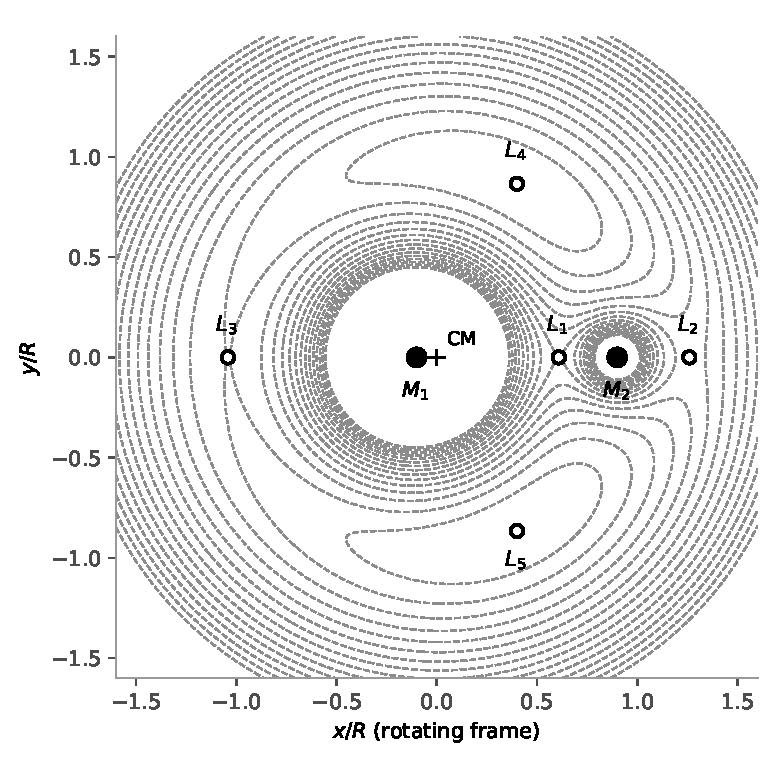
\includegraphics[width=3.6in]{ueff_contours}
  \caption{Contours of the effective potential $\Ueff$ in the rotating frame for $\mu = 0.1$,
    with the two primaries (filled) and the five Lagrange points (open). $L_1$, $L_2$, $L_3$
    are saddle points; $L_4$ and $L_5$ are the two maxima. Drawn by \texttt{make\_figure.py}
    in the handout's folder.}
  \label{fig:ueff}
\end{figure}

\medskip

\noindent\textbf{Board problem (a): $L_4$ and $L_5$.} Show that the two points forming
equilateral triangles with $M_1$ and $M_2$ satisfy \eqref{eq:equilibrium}, whatever the mass
ratio. Work with the forces per unit mass, and use \eqref{eq:kepler} and the fact that the CM
is at the origin.

\solution{The equation to check is \eqref{eq:equilibrium}, $\grad{\Ueff} = 0$. Divided by $m$
and with $\Ueff = U - \tfrac12 m\Om^2(x^2+y^2)$ written out, it says
$-\tfrac{1}{m}\grad{U} + \Om^2\vr = 0$: gravity per unit mass plus the centrifugal force per
unit mass must vanish. Let $\vr$ be such a point and $\vr_1$, $\vr_2$ the primaries. By construction
$|\vr - \vr_1| = |\vr - \vr_2| = R$. Each primary pulls with magnitude $GM_i/R^2$ along the unit
vector $(\vr_i - \vr)/R$ toward it (a unit vector because the distance is $R$), so gravity per
unit mass is the sum of two (magnitude)$\times$(unit vector) terms,
\begin{align}
  -\frac{1}{m}\grad{U} &= \frac{GM_1}{R^2}\,\frac{\vr_1 - \vr}{R} + \frac{GM_2}{R^2}\,\frac{\vr_2 - \vr}{R}
  = \frac{GM_1(\vr_1 - \vr)}{R^3} + \frac{GM_2(\vr_2 - \vr)}{R^3} \nonumber\\
  &= \frac{G}{R^3}\Bigl[(M_1\vr_1 + M_2\vr_2) - (M_1+M_2)\,\vr\Bigr]
  = \frac{G}{R^3}\Bigl[(M_1+M_2)\,\mathbf{r}_{\rm cm} - (M_1+M_2)\,\vr\Bigr] \nonumber\\
  &= -\frac{G(M_1+M_2)}{R^3}\,\vr = -\Om^2\vr ,
\end{align}
because $\mathbf{r}_{\rm cm} \equiv (M_1\vr_1 + M_2\vr_2)/(M_1+M_2)$ (the definition of the CM) is
$0$, the CM being at the origin, and the last step is \eqref{eq:kepler}. The centrifugal force per
unit mass is $+\Om^2\vr$ (the $m\Om^2(x,y)$ of \eqref{eq:eom}, divided by $m$). They cancel, so
\eqref{eq:equilibrium} holds. In words: at the equilateral points the two bodies' gravity
points exactly at the CM, with exactly the strength a circular orbit of angular speed $\Om$
needs at that radius, so the test mass goes around the CM in step with the primaries. The
dashed triangle in the diagram of the setup is this point.}

\medskip

\noindent\textbf{Another route, for a group that finishes early: polar coordinates.} Put the
test mass at $(r, \theta)$ from the CM, with $\theta$ measured from the CM-to-$M_2$ line, so the
distances to the primaries are $r_1' = \sqrt{r^2 + 2 r r_1\cos\theta + r_1^2}$ and
$r_2' = \sqrt{r^2 - 2 r r_2\cos\theta + r_2^2}$ (law of cosines; $M_1$ is at angle $\pi$, $M_2$ at
angle $0$) with $r_1 = \mu R$, $r_2 = (1-\mu)R$. The
centrifugal term depends on $r$ alone, so the $\theta$ half of \eqref{eq:equilibrium} is
$\partial U/\partial\theta = 0$. Since $\partial r_1'/\partial\theta = -r r_1\sin\theta/r_1'$ and
$\partial r_2'/\partial\theta = +r r_2\sin\theta/r_2'$, and since
$U = -GmM_1/r_1' - GmM_2/r_2'$ gives, by the chain rule,
$\partial U/\partial\theta = (GmM_1/r_1'^2)\,\partial r_1'/\partial\theta
+ (GmM_2/r_2'^2)\,\partial r_2'/\partial\theta$, we get
$\partial U/\partial\theta = -GmM_1 r r_1\sin\theta/r_1'^3 + GmM_2 r r_2\sin\theta/r_2'^3$, and
because $M_1 r_1 = M_2 r_2$ (the CM condition from the setup) it factors:
\begin{equation}
  \pd{U}{\theta} = G m\, r\, M_1 r_1 \sin\theta\,\Bigl(\frac{1}{r_2'^3} - \frac{1}{r_1'^3}\Bigr) = 0 .
\end{equation}
So every equilibrium has $\sin\theta = 0$ (on the axis: $L_1$, $L_2$, $L_3$, one in each of the three stretches the primaries cut
the axis into, as ``The exact positions'' below shows) or $r_1' = r_2'$
(on the perpendicular bisector of the primaries: $L_4$, $L_5$), and nothing else. On the
bisector $r_1' = r_2' \equiv s$, and the algebra of (a) goes through with $R$ replaced by $s$:
gravity per unit mass is $-G(M_1+M_2)\vr/s^3$, pointing at the CM, against the centrifugal
$+\Om^2\vr = +G(M_1+M_2)\vr/R^3$. So the $r$ half of \eqref{eq:equilibrium} holds only at
$s = R$, the equilateral point. This factorization is the quickest
way to see that there are exactly five points. (It is how Edlund, Am.\ J.\ Phys.\ \textbf{92},
414 (2024), organizes the whole problem.)

\medskip

\noindent\textbf{Board problem (b): $L_1$ and $L_2$ for a small $\mu$.} Use units with $R = 1$
and $G(M_1+M_2) = 1$, so $\Om = 1$ by \eqref{eq:kepler}, $M_1 \to 1-\mu$ at $x = -\mu$ and
$M_2 \to \mu$ at $x = 1-\mu$. On the axis $y = 0$ the $y$ half of \eqref{eq:equilibrium} holds automatically
($\partial U/\partial y$ and $m\Om^2 y$ both carry a factor of $y$), and the $x$ half is
\begin{equation}
  \label{eq:axis}
  x = \frac{(1-\mu)(x+\mu)}{|x+\mu|^3} + \frac{\mu\,(x-1+\mu)}{|x-1+\mu|^3} .
\end{equation}
(This is $-\partial\Ueff/\partial x = 0$ per unit mass at $y = 0$, with the centrifugal term
$\Om^2 x = x$ on the left and the two gravitational pulls, $-GM_i(x - x_i)/|x - x_i|^3$ toward
$M_i$ at $x_i$, moved to the right.) Show that for
$\mu \ll 1$ both $L_1$ and $L_2$ sit a distance
\begin{equation}
  \label{eq:hill}
  d \approx R\,\Bigl(\frac{\mu}{3}\Bigr)^{1/3}
\end{equation}
from $M_2$, one on each side, and evaluate it for the Sun and the Earth ($\mu = 3.00\times
10^{-6}$, $R = 1.496\times 10^8$~km). This $d$ is called the \emph{Hill radius}; inside it
$M_2$'s gravity wins over $M_1$'s tidal pull plus the centrifugal force (the $-2\delta$ and the
$+\delta$ in the solution below), which is why the Moon is Earth's.

\solution{Take $L_2$ first: $x = 1 - \mu + \delta$ with $\delta > 0$ (beyond $M_2$). Keep
first order in $\delta$, drop $\mu$ wherever it is added to a number of order one, but keep
$\mu/\delta^2$, which is the term that matters. (This is consistent because the answer has
$\delta \sim \mu^{1/3}$: then $\mu \ll \delta$, while $\mu/\delta^2 \sim \delta$.) The left side of \eqref{eq:axis} is $1 +
\delta$; the first term on the right is $(1-\mu)/(1+\delta)^2 \approx 1 - 2\delta$ (here $x + \mu = 1 + \delta$; binomial expansion $(1+\delta)^{-2} \approx 1 - 2\delta$, and
the factor $1 - \mu$ becomes $1$); the second is $\mu\delta/\delta^3 = \mu/\delta^2$ (here
$x - 1 + \mu = \delta$). So
\begin{equation}
  1 + \delta \approx 1 - 2\delta + \frac{\mu}{\delta^2}
  \quad\Rightarrow\quad 3\delta = \frac{\mu}{\delta^2}
  \quad\Rightarrow\quad \delta^3 = \frac{\mu}{3} .
\end{equation}
For $L_1$ put $x = 1 - \mu - \delta$: the left side is $1 - \delta$, the first term is
$(1-\mu)/(1-\delta)^2 \approx 1 + 2\delta$, and the second is $\mu(-\delta)/\delta^3 =
-\mu/\delta^2$, so $1 - \delta \approx 1 + 2\delta - \mu/\delta^2$, giving
$-3\delta = -\mu/\delta^2$ and the same $\delta$. To this order $L_1$
and $L_2$ are mirror images about $M_2$, and with $R$ restored, $d = \delta R = R(\mu/3)^{1/3}$,
which is \eqref{eq:hill}. For the Sun and the Earth, $(\mu/3)^{1/3} =
(1.00\times 10^{-6})^{1/3} = 0.0100$, so $d = 0.0100\;\mathrm{AU} = 1.50\times 10^6$~km, about
four times the Moon's distance. JWST orbits around $L_2$ (a ``halo orbit'' a few hundred
thousand km across), so that it always has the Sun, the Earth and the Moon on the same side,
behind its sunshield.}

\medskip

\noindent\textbf{The exact positions.} Equation \eqref{eq:axis} is a quintic once the absolute
values are resolved, so the three collinear points are found numerically. There is exactly one in each of the
intervals below: for $f$ in the code (left side of \eqref{eq:axis} minus right side),
$f'(x) = 1 + 2(1-\mu)/|x+\mu|^3 + 2\mu/|x-1+\mu|^3 > 0$, and $f$ runs from $-\infty$ to
$+\infty$ across each interval. Solving it with
\texttt{scipy.optimize.brentq} on the three intervals (left of $M_1$, between, right of
$M_2$):

\begin{center}
\small
\begin{tabular}{lrrrrr}
\toprule
 & $\mu$ & $L_1$: inside $M_2$ & $L_2$: beyond $M_2$ & $d$ from \eqref{eq:hill} & $L_3$, $x/R$ \\
\midrule
Sun--Earth    & $3.00\times 10^{-6}$ & $1.49\times 10^6$ km & $1.50\times 10^6$ km & $1.50\times 10^6$ km & $-1.000001$ \\
Sun--Jupiter  & $9.54\times 10^{-4}$ & $5.19\times 10^7$ km & $5.43\times 10^7$ km & $5.31\times 10^7$ km & $-1.0004$ \\
Earth--Moon   & $1.22\times 10^{-2}$ & $5.80\times 10^4$ km & $6.45\times 10^4$ km & $6.13\times 10^4$ km & $-1.005$ \\
\bottomrule
\end{tabular}
\end{center}

\noindent The approximation \eqref{eq:hill} is good to about a third of a percent for the Earth and
to about five percent for the Moon, whose $\mu$ is not so small (the next term in the
expansion is of relative size $\mp\frac13(\mu/3)^{1/3}$). $L_3$ sits on the far side of
$M_1$, essentially on $M_2$'s orbit. The code is a few lines:
\begin{verbatim}
from scipy.optimize import brentq
def f(x, mu):
    return x - (1-mu)*(x+mu)/abs(x+mu)**3 - mu*(x-1+mu)/abs(x-1+mu)**3
mu = 3.003e-6
L3 = brentq(f, -2.0, -mu-1e-9, args=(mu,))
L1 = brentq(f, -mu+1e-9, 1-mu-1e-9, args=(mu,))
L2 = brentq(f, 1-mu+1e-9, 2.5, args=(mu,))
\end{verbatim}

\medskip

\noindent\textbf{Noether again: the Jacobi integral.} $\Lag$ in \eqref{eq:Lrot} has no explicit
$t$, so Section~7.8 says $\Ham = p_x\dot x + p_y\dot y - \Lag$ is conserved. With $p_x =
m(\dot x - \Om y)$ and $p_y = m(\dot y + \Om x)$,
\begin{align}
  \Ham &= m(\dot x - \Om y)\,\dot x + m(\dot y + \Om x)\,\dot y - \Lag
  = m(\dot x^2 + \dot y^2) + m\Om(x\dot y - y\dot x) - \Lag \nonumber\\
  &= m(\dot x^2 + \dot y^2) + m\Om(x\dot y - y\dot x) \nonumber\\
  &\qquad - \Bigl[\tfrac12 m(\dot x^2 + \dot y^2) + m\Om(x\dot y - y\dot x)
  + \tfrac12 m\Om^2(x^2 + y^2) - U\Bigr] \nonumber\\
  &= \tfrac12 m(\dot x^2 + \dot y^2) + \Ueff(x,y) .
  \label{eq:jacobi}
\end{align}
(Subtracting \eqref{eq:Lrot}, the $m\Om(x\dot y - y\dot x)$ terms cancel, half of
$m(\dot x^2 + \dot y^2)$ is left, and $\tfrac12 m\Om^2(x^2+y^2) - U$ comes in with its sign
flipped, which is $\Ueff$.) This is the Jacobi integral (celestial mechanics usually quotes $C_J = -2\Ham/m$). Three
remarks, the first two of which are the point of Section~7.8:
\begin{enumerate}
\item It is conserved, and it looks like an energy: kinetic energy in the rotating frame plus
  the effective potential.
\item It is \emph{not} $T + U$. The true kinetic energy is $\tfrac12 m(\dot X^2 + \dot Y^2)$,
  and from Step~1 it is $\tfrac12 m(\dot x^2 + \dot y^2) + m\Om(x\dot y - y\dot x)
  + \tfrac12 m\Om^2(x^2+y^2)$; adding $U$ and subtracting \eqref{eq:jacobi},
  \begin{align}
    T + U - \Ham &= \Bigl[\tfrac12 m(\dot x^2 + \dot y^2) + m\Om(x\dot y - y\dot x)
      + \tfrac12 m\Om^2(x^2+y^2) + U\Bigr] \nonumber\\
    &\qquad - \Bigl[\tfrac12 m(\dot x^2 + \dot y^2) + U - \tfrac12 m\Om^2(x^2+y^2)\Bigr]
    = m\Om(x\dot y - y\dot x) + m\Om^2(x^2 + y^2),
  \end{align}
  which is not constant: in polar coordinates it is $\Om\, m r^2(\dot\theta + \Om)$, $\Om$ times
  $m$'s angular momentum about the CM in the inertial frame (whose angular velocity is
  $\dot\theta + \Om$), and the primaries' pull is not aimed at the CM, so it exerts a torque. Taylor's condition for $\Ham = T + U$ (Section~7.8, pp.~269--272) was that the relation between
  the generalized coordinates and the inertial position not involve $t$; \eqref{eq:rotation}
  involves $t$, so the condition fails, exactly as for the spinning hoop. (And $T + U$ is not
  conserved in the inertial frame either: there the primaries move and $U$ depends on time.
  The symmetry lives in the rotating frame, and so does the conservation
  law.)\footnote{This is easy to get wrong in print. Edlund's paper (cited in the polar-coordinates paragraph) calls $\Ueff$
    ``devoid of physical meaning'' because it seems to assume the body's angular velocity is
    constant, and proposes that the test mass's angular momentum is conserved ``regionally''
    near each Lagrange point. Neither is needed. The $\Om$ in $\Ueff$ is the \emph{frame's}
    rotation rate, constant by construction; the body's own angular velocity varies, and
    \eqref{eq:Lrot} carries that in the kinetic and Coriolis terms. $\Ham$ in \eqref{eq:jacobi}
    is conserved exactly, everywhere, for the reason in Section~7.8: no $t$ in $\Lag$. The
    puzzle comes from expecting a two-body potential $L^2/2mr^2$ with $L$ the test mass's
    angular momentum, which is not conserved here and is not used.}
\item Since $\tfrac12 m v_{\rm rot}^2 \geq 0$, a body with a given $\Ham$ can only be where
  $\Ueff \leq \Ham$. The contours in Figure~\ref{fig:ueff} are therefore fences (Hill's
  \emph{zero-velocity curves}): a satellite with $\Ham$ below $\Ueff(L_1)$ that starts near
  $M_2$ can never leave $M_2$'s neighbourhood, however it moves. Raising $\Ham$ past
  $\Ueff(L_1)$ opens a gate to $M_1$; past $\Ueff(L_2)$, a gate to the outside.
\end{enumerate}

\medskip

\noindent\textbf{Stability, in one paragraph (not derived today).} $L_1$, $L_2$ and $L_3$ are
saddle points of $\Ueff$ and are unstable: JWST fires its thrusters every few weeks to stay
near $L_2$. $L_4$ and $L_5$ are \emph{maxima} of $\Ueff$, and yet they are stable whenever
$27\mu(1-\mu) < 1$ (a quoted result, Gascheau's of 1843; Murray and Dermott, Chapter~3, derive
it), i.e.\ $\mu < 0.0385$, which covers Sun--Jupiter (the Trojans) and
Earth--Moon. A stable equilibrium at a potential maximum is impossible for a static potential:
the small-oscillation analysis of Taylor's Example~7.7 would call it unstable. What rescues it
is the Coriolis force, which does no work but keeps turning the velocity, so a body that starts
to fall off the hill is swung around it instead (Greenberg and Davis, ``Stability at potential maxima,'' Am.\ J.\
Phys.\ \textbf{46}, 1068 (1978)). Showing that means linearizing
\eqref{eq:eom} \emph{with} the velocity terms kept, a $4\times 4$ eigenvalue problem; it is a
very good project, and the same velocity-coupled linear equations appear in Chapter~9's
Foucault pendulum.

\section{The Lagrange points, straight through}
\label{sec:straight}

Section~\ref{sec:lagrange} is the long version. This section is the same problem done the way
every Chapter~7 problem is done, in the order of Section~7.5's recipe (p.~258) and
Examples~7.4--7.7: set the problem up, write the Lagrangian with nothing left out, state the
constraints, write the Lagrangian with the constraints in, take Lagrange's equations, read off
what they say. Every step is here. Where Section~\ref{sec:lagrange} did a piece of algebra at
length, the result is quoted by equation number and the line or two that produce it are shown.

\medskip

\noindent\textbf{The idea in one paragraph.} The inertial coordinates $(X, Y)$ are the
ordinary, time-independent ones; the trouble is that in them the Lagrangian carries $t$
explicitly, because the primaries move and so $U(X, Y, t)$ changes in time, and neither of
Chapter~7's tests (an ignorable coordinate, Section~7.6; no explicit $t$, Section~7.8) finds a
conserved quantity. The move is to change to rotating coordinates $(x, y)$, which are
themselves time-dependent functions of $(X, Y)$, the kind of generalized coordinate
Section~7.3 allows and Example~7.6's spinning hoop uses. In them the primaries sit still, so
$U(x, y)$ has no $t$, and the Hamiltonian is conserved: that is the Jacobi integral. The price
of time-dependent coordinates is that they are not ``natural'' (Section~7.3), so $T$ picks up
terms linear in the velocities and a velocity-free term, and the conserved $\Ham$ is not
$T + U$ (Section~7.8). The redshift problem of Sections~\ref{sec:redshift}
and~\ref{sec:redshift-straight} is the mirror image: the comoving coordinate $x = r/a(t)$ is
also a time-dependent change, and it makes $x$ ignorable, but $t$ survives in $\Lag$ through
$a(t)$, so there the Hamiltonian is not conserved. One problem gains a conserved $\Ham$ from
the change of coordinates; the other does not.

\medskip

\noindent\textbf{Step 1: set up the problem.} Two bodies $M_1$ and $M_2$ (the primaries), a
distance $R$ apart, go around their centre of mass (CM) in circles at angular speed $\Om$; a
third body of mass $m$ moves in their gravity. Put the origin at the CM and use inertial
Cartesian coordinates $(X, Y, Z)$ with the primaries' orbit in the plane $Z = 0$. At time $t$
the primaries are at
\begin{equation}
  \label{eq:primaries}
  \begin{gathered}
  \vr_1(t) = r_1(-\cos\Om t,\, -\sin\Om t,\, 0), \qquad
  \vr_2(t) = r_2(\cos\Om t,\, \sin\Om t,\, 0), \\
  r_1 = \frac{M_2 R}{M_1 + M_2},\quad r_2 = \frac{M_1 R}{M_1 + M_2},
  \end{gathered}
\end{equation}
on opposite sides of the CM: ``origin at the CM'' means $M_1\vr_1 + M_2\vr_2 = 0$, i.e.\ $M_1 r_1 = M_2 r_2$ (the bodies are on opposite sides);
putting $r_2 = R - r_1$ into it gives $(M_1 + M_2)\,r_1 = M_2 R$, and likewise for $r_2$. Newton's second law for $M_1$ fixes the rate: its acceleration is $\Om^2 r_1$ toward the CM
(uniform circular motion) and the only force on it is $M_2$'s pull $GM_1M_2/R^2$, also toward
the CM, so $M_1\Om^2 r_1 = GM_1M_2/R^2$; with $r_1$ from \eqref{eq:primaries} this is
$M_1M_2\Om^2 R/(M_1+M_2) = GM_1M_2/R^2$, and cancelling $M_1M_2$ and multiplying by
$(M_1+M_2)/R$,
\begin{equation}
  \label{eq:kepler3}
  \Om^2 = \frac{G(M_1 + M_2)}{R^3},
\end{equation}
Kepler's third law for the pair (this is \eqref{eq:kepler}).

\medskip

\noindent\textbf{Step 2: the Lagrangian, with nothing left out.} The body $m$ has three
Cartesian coordinates and, so far, no constraint, so as in Section~7.1 for a single particle,
$\Lag = T - U$ with
\begin{equation}
  \label{eq:L3d}
  \Lag = \tfrac12 m\bigl(\dot X^2 + \dot Y^2 + \dot Z^2\bigr) - U(X, Y, Z, t), \qquad
  U = -\frac{GmM_1}{|\vr - \vr_1(t)|} - \frac{GmM_2}{|\vr - \vr_2(t)|},
\end{equation}
where $|\vr - \vr_i(t)| = \sqrt{(X - X_i(t))^2 + (Y - Y_i(t))^2 + Z^2}$ and $(X_i, Y_i)$ are
the components in \eqref{eq:primaries}. Lagrange's equations for $X$, $Y$ and $Z$ are Newton's
second law with the two attractions: for $X$, $\partial\Lag/\partial\dot X = m\dot X$ and
$\partial\Lag/\partial X = -\partial U/\partial X$, so
$\frac{d}{dt}\partial\Lag/\partial\dot X = \partial\Lag/\partial X$ reads
$m\ddot X = -\partial U/\partial X$, and likewise for $Y$ and $Z$; together,
$m\ddot{\vr} = -\grad U$. Neither of Chapter~7's tests finds a conserved quantity as it stands: $t$ appears explicitly through
$\vr_1(t)$ and $\vr_2(t)$, so Section~7.8's $\Ham$ is not constant, and no coordinate is
ignorable (Section~7.6), since $U$ depends on all three.

\medskip

\noindent\textbf{Step 3: the constraints.} Two things are being held fixed. It pays to say
which kind of ``held fixed'' each one is.

\smallskip
\noindent (i) \emph{The primaries' motion is prescribed.} $\vr_1(t)$ and $\vr_2(t)$ are given
functions of $t$, not coordinates to be varied: $m$ is taken too small to disturb them (the
restricted three-body problem; the footnote in Section~\ref{sec:lagrange}). This is the same
move as Example~7.6, the bead on a spinning hoop, where the hoop's angle $\omega t$ is
prescribed and only the bead's $\theta$ is a coordinate. It is a constraint on the system, not
on $m$: it removes the six coordinates of the primaries from the problem and is what put $t$
into $U$.

\smallskip
\noindent (ii) \emph{Motion in the orbital plane.} Set $Z = 0$. This is not a constraint in
Section~7.3's sense, since no wire or surface enforces it. It is a choice of initial conditions
that the equations of motion respect: $U$ is even in $Z$ (both distances contain $Z$ only as
$Z^2$), so $\partial U/\partial Z = GmM_1 Z/|\vr - \vr_1|^3 + GmM_2 Z/|\vr - \vr_2|^3$, which is $0$ on $Z = 0$, and the $Z$ equation
$m\ddot Z = -\partial U/\partial Z$ gives $\ddot Z = 0$ there. A body that starts in the plane
with $\dot Z = 0$ stays in it, and we look only at those motions.

\smallskip
\noindent So once the primaries are prescribed, $m$ has three degrees of freedom; restricting
to the planar motions of (ii) removes $Z$ and does nothing to $X$ and $Y$. Two generalized
coordinates remain.

\medskip

\noindent\textbf{Step 4: the Lagrangian with the constraints in, in good coordinates.} With
$Z = 0$ the Lagrangian \eqref{eq:L3d} loses its $\dot Z$ term and $U$ loses $Z$:
\begin{equation}
  \label{eq:L2d}
  \Lag = \tfrac12 m\bigl(\dot X^2 + \dot Y^2\bigr) - U(X, Y, t).
\end{equation}
The only question Chapter~7 leaves open is which two generalized coordinates to use. $U$
depends on $t$ only because the primaries move, so in coordinates that turn with them it will
not. Section~7.3 allows generalized coordinates whose relation to the position involves $t$
(Example~7.6 uses one), so take the rotating coordinates
\eqref{eq:rotation}, $X = x\cos\Om t - y\sin\Om t$, $Y = x\sin\Om t + y\cos\Om t$. In them the
primaries sit at $(x, y) = (-r_1, 0)$ and $(r_2, 0)$ for all time (put $(x,y) = (r_2, 0)$ into
the rotation: $X = r_2\cos\Om t$, $Y = r_2\sin\Om t$, which is \eqref{eq:primaries}; $(-r_1, 0)$ likewise gives $\vr_1(t)$), so
\begin{equation}
  \label{eq:U2d}
  U(x, y) = -\frac{GmM_1}{\sqrt{(x + r_1)^2 + y^2}} - \frac{GmM_2}{\sqrt{(x - r_2)^2 + y^2}},
\end{equation}
with no $t$. For the kinetic energy, differentiate the rotation with the product rule ($\Om$
constant) and collect the $\cos\Om t$ and $\sin\Om t$ terms, which is \eqref{eq:XYdot}:
$\dot X = (\dot x - \Om y)\cos\Om t - (\dot y + \Om x)\sin\Om t$ and
$\dot Y = (\dot x - \Om y)\sin\Om t + (\dot y + \Om x)\cos\Om t$. Square and add: the cross
terms $\mp 2(\dot x - \Om y)(\dot y + \Om x)\sin\Om t\cos\Om t$ cancel and
$\cos^2\Om t + \sin^2\Om t = 1$, so $\dot X^2 + \dot Y^2 = (\dot x - \Om y)^2 + (\dot y + \Om x)^2$,
and expanding the squares (as in \eqref{eq:speed}),
$\dot X^2 + \dot Y^2 = \dot x^2 + \dot y^2 + 2\Om(x\dot y - y\dot x) + \Om^2(x^2 + y^2)$;
putting $\tfrac12 m$ times this into \eqref{eq:L2d},
\begin{equation}
  \label{eq:Lrot3}
  \boxed{\;\Lag = \tfrac12 m(\dot x^2 + \dot y^2) + m\Om\,(x\dot y - y\dot x)
  + \tfrac12 m\Om^2(x^2 + y^2) - U(x, y)\;}
\end{equation}
which is \eqref{eq:Lrot}. Two remarks before differentiating. There is no explicit $t$ in $\Lag$
any more; that was the point of the coordinate change. And the coordinates are not
``natural'' in Section~7.3's sense: the relation between $(x, y)$ and $(X, Y)$ involves $t$, so
$T$ is not a pure quadratic in $\dot x, \dot y$ (there are the linear terms $m\Om(x\dot y -
y\dot x)$ and the velocity-free term $\tfrac12 m\Om^2(x^2 + y^2)$), exactly as for the bead on
the spinning hoop.

\medskip

\noindent\textbf{Step 5: Lagrange's equations.} From \eqref{eq:Lrot3},
\begin{align*}
  \pd{\Lag}{\dot x} &= m(\dot x - \Om y), &
  \pd{\Lag}{x} &= m\Om\dot y + m\Om^2 x - \pd{U}{x}, \\
  \pd{\Lag}{\dot y} &= m(\dot y + \Om x), &
  \pd{\Lag}{y} &= -m\Om\dot x + m\Om^2 y - \pd{U}{y}.
\end{align*}
With $\Om$ constant, $\frac{d}{dt}\,m(\dot x - \Om y) = m\ddot x - m\Om\dot y$ and
$\frac{d}{dt}\,m(\dot y + \Om x) = m\ddot y + m\Om\dot x$, so
$\frac{d}{dt}\partial\Lag/\partial\dot q = \partial\Lag/\partial q$ for $q = x$ and $q = y$
reads
\begin{align*}
  m\ddot x - m\Om\dot y &= m\Om\dot y + m\Om^2 x - \pd{U}{x}, \\
  m\ddot y + m\Om\dot x &= -m\Om\dot x + m\Om^2 y - \pd{U}{y}.
\end{align*}
Move the $-m\Om\dot y$ and the $+m\Om\dot x$ from the left to the right, where each doubles its
partner:
\begin{equation}
  \label{eq:eom3}
  m\ddot x = -\pd{U}{x} + m\Om^2 x + 2m\Om\dot y, \qquad
  m\ddot y = -\pd{U}{y} + m\Om^2 y - 2m\Om\dot x ,
\end{equation}
which is \eqref{eq:eom}: gravity, then a centrifugal force $m\Om^2(x, y)$ pointing away from
the axis, then a Coriolis force $2m\Om(\dot y, -\dot x)$ perpendicular to the velocity.
Chapter~9 will derive both from Newton's second law in a rotating frame; here they came out of
Lagrange's equations because the coordinates rotate.

\medskip

\noindent\textbf{Step 6: read off results.} Two, each one line of reasoning from
\eqref{eq:Lrot3} or \eqref{eq:eom3}.

\smallskip
\noindent (a) \emph{Where can $m$ sit still?} ``Sit still in the rotating frame'' means
$\dot x = \dot y = 0$ and $\ddot x = \ddot y = 0$. Put those into \eqref{eq:eom3}: the Coriolis
terms vanish with the velocities, the left sides vanish with the accelerations, and
\begin{equation}
  \label{eq:equilibrium3}
  0 = -\pd{U}{x} + m\Om^2 x, \qquad 0 = -\pd{U}{y} + m\Om^2 y,
  \qquad\text{i.e.}\qquad \grad\Ueff = 0,\quad \Ueff \equiv U - \tfrac12 m\Om^2(x^2 + y^2),
\end{equation}
since $m\Om^2 x = -\partial_x\bigl(-\tfrac12 m\Om^2(x^2 + y^2)\bigr)$ and likewise for $y$.
This has five solutions: three on the $x$ axis ($L_1$, $L_2$, $L_3$; the equation
\eqref{eq:axis} and the table in Section~\ref{sec:lagrange}) and two off it, and no others (the polar-coordinates paragraph of Section~\ref{sec:lagrange});
Figure~\ref{fig:fivepoints} shows all five. The two off it take three lines. With $\vr = (x, y)$ and $\vr_1 = (-r_1, 0)$, $\vr_2 = (r_2, 0)$ the rotating-frame positions, at a
point $\vr$ a distance $R$ from \emph{both} primaries (the third corner
of an equilateral triangle on $M_1M_2$), each primary pulls with magnitude $GM_i/R^2$ along the
unit vector $(\vr_i - \vr)/R$, so, dividing \eqref{eq:equilibrium3} by $m$ and writing the
gravity term as (magnitude)$\times$(unit vector),
\begin{align}
  -\frac1m\grad U &= \frac{GM_1}{R^2}\,\frac{\vr_1 - \vr}{R} + \frac{GM_2}{R^2}\,\frac{\vr_2 - \vr}{R}
  = \frac{GM_1(\vr_1 - \vr)}{R^3} + \frac{GM_2(\vr_2 - \vr)}{R^3} \nonumber\\
  &= \frac{G}{R^3}\Bigl[(M_1\vr_1 + M_2\vr_2) - (M_1 + M_2)\,\vr\Bigr]
  = -\frac{G(M_1 + M_2)}{R^3}\,\vr = -\Om^2\vr ,
\end{align}
using $M_1\vr_1 + M_2\vr_2 = 0$ (origin at the CM) and then \eqref{eq:kepler3}; the
centrifugal term of \eqref{eq:equilibrium3} divided by $m$ is $+\Om^2\vr$, and the two cancel.
Those are $L_4$ and $L_5$, $60^\circ$ ahead of and behind $M_2$ as seen from $M_1$, for any mass
ratio (on $M_2$'s orbit only in the limit $\mu \to 0$). (Jupiter's Trojans.)

\begin{figure}[htb]
  \centering
  \begin{tikzpicture}[scale=3.0]
    \draw[->, gray] (-1.35,0) -- (1.55,0) node[below right] {$x$};
    \draw[->, gray] (0,-1.1) -- (0,1.1) node[left] {$y$};
    \draw[dashed, gray] (0,0) circle (0.9);
    \draw[dashed] (-0.1,0) -- (0.4,0.866) -- (0.9,0) -- (0.4,-0.866) -- cycle;
    \fill (-0.1,0) circle (0.055) node[below left=2pt] {$M_1$};
    \fill (0.9,0) circle (0.03) node[below=3pt] {$M_2$};
    \draw[thick] (-0.03,0) -- (0.03,0) (0,-0.03) -- (0,0.03);
    \draw (0.16,0.11) node {\scriptsize CM} -- (0.03,0.02);
    \foreach \x/\lab/\pos in {0.609/L_1/above, 1.2597/L_2/below, -1.0416/L_3/above}
      \draw (\x,0) circle (0.025) node[\pos=2pt] {$\lab$};
    % a satellite at L2 (JWST), leader line down to the point
    \draw[gray] (1.2597,0.03) -- (1.2597,0.17);
    \begin{scope}[shift={(1.2597,0.27)}, scale=0.045, rotate=15]
      \draw[thick] (-4,0) -- (4,0);
      \fill (-4,-0.7) rectangle (-1.4,0.7);
      \fill (1.4,-0.7) rectangle (4,0.7);
      \fill (-1.1,-1.1) rectangle (1.1,1.1);
      \draw[thick] (0,1.1) -- (0,2.2);
      \draw[thick] (-1.2,2.2) arc (180:360:1.2 and 0.5);
    \end{scope}
    \draw (0.4,0.866) circle (0.025) node[above=2pt] {$L_4$};
    \draw (0.4,-0.866) circle (0.025) node[below=2pt] {$L_5$};
  \end{tikzpicture}
  \caption{The five Lagrange points in the rotating frame, drawn to scale for
    $\mu = M_2/(M_1+M_2) = 0.1$ (the mass ratio of Figure~\ref{fig:ueff}; for the Sun and the
    Earth, $L_1$ and $L_2$ sit one percent of $R$ from the Earth and would not separate on the
    page). $L_1$, $L_2$, $L_3$ on the line of the primaries, found from \eqref{eq:axis};
    $L_4$, $L_5$ at the third corners of the two equilateral triangles (dashed) on $M_1M_2$.
    The dashed circle is $M_2$'s orbit about the CM. The satellite marks $L_2$: for the Sun and
    the Earth that is where JWST sits, beyond the Earth on the far side from the Sun (SOHO sits
    at $L_1$); the Trojan asteroids are at $L_4$ and $L_5$.}
  \label{fig:fivepoints}
\end{figure}

\smallskip
\noindent (b) \emph{What is conserved?} $\Lag$ in \eqref{eq:Lrot3} has no explicit $t$, so by
Section~7.8 the Hamiltonian $\Ham = \sum_i p_i\dot q_i - \Lag$ is conserved. With
$p_x = \partial\Lag/\partial\dot x = m(\dot x - \Om y)$ and
$p_y = \partial\Lag/\partial\dot y = m(\dot y + \Om x)$,
\begin{align}
  \Ham &= m(\dot x - \Om y)\dot x + m(\dot y + \Om x)\dot y - \Lag
  = m(\dot x^2 + \dot y^2) + m\Om(x\dot y - y\dot x) - \Lag \nonumber\\
  &= m(\dot x^2 + \dot y^2) + m\Om(x\dot y - y\dot x) \nonumber\\
  &\qquad - \Bigl[\tfrac12 m(\dot x^2 + \dot y^2) + m\Om(x\dot y - y\dot x)
  + \tfrac12 m\Om^2(x^2 + y^2) - U\Bigr] \nonumber\\
  &= \tfrac12 m(\dot x^2 + \dot y^2) + \Ueff(x, y),
  \label{eq:jacobi3}
\end{align}
the last line by subtracting \eqref{eq:Lrot3} term by term: the $m\Om(x\dot y - y\dot x)$
cancel, half of $m(\dot x^2 + \dot y^2)$ survives, and $-\tfrac12 m\Om^2(x^2+y^2) + U$ is
$\Ueff$. This is the Jacobi integral. It is \emph{not} $T + U$ (Section~7.8 said it would not
be, because the coordinate relation involves $t$), and it is more useful than $T + U$ would be:
since $\tfrac12 m(\dot x^2 + \dot y^2) \ge 0$, a body with a given $\Ham$ can only be where
$\Ueff(x, y) \le \Ham$. A moon with $\Ham$ below the value of $\Ueff$ at $L_1$ that starts near its planet can never leave
its planet's neighbourhood, however it moves inside it.

\smallskip
\noindent That is the whole calculation. Section~\ref{sec:lagrange} adds the diagram, the
numbers, the polar-coordinate route, and the question of stability, which needs the Coriolis
term kept.

\end{document}
